\documentclass[12pt,a4paper]{article}
\usepackage{fontspec}
\setmainfont{Times New Roman}
\setsansfont{Arial}
\setmonofont{Consolas}[Scale=0.85]
\usepackage[left=2.7cm,right=2.3cm,top=2.5cm,bottom=2.5cm]{geometry}
\usepackage{amsmath,amssymb,booktabs,array,tabularx,longtable}
\usepackage{graphicx,float,setspace,enumitem,xcolor,fancyhdr}
\usepackage{caption}
\usepackage{xurl}
\usepackage[colorlinks=true,linkcolor=blue!45!black,citecolor=blue!45!black,urlcolor=blue!45!black]{hyperref}
\hypersetup{pdftitle={Phân tích dữ liệu cảm biến và dự đoán RUL trên NASA C-MAPSS FD001},pdfauthor={}}
\renewcommand{\contentsname}{Mục lục}
\renewcommand{\listfigurename}{Danh mục hình}
\renewcommand{\listtablename}{Danh mục bảng}
\renewcommand{\figurename}{Hình}
\renewcommand{\tablename}{Bảng}
\renewcommand{\refname}{Tài liệu tham khảo}
\newcommand{\reportdate}{22/09/2026}
\newcommand{\filepath}[1]{\nolinkurl{#1}}
\newcolumntype{L}[1]{>{\raggedright\arraybackslash}p{#1}}
\onehalfspacing
\setlength{\parindent}{0.7cm}
\setlength{\emergencystretch}{2em}
\setlength{\headheight}{16pt}
\setlist{nosep,leftmargin=*}
\captionsetup{font=small,labelfont=bf}
\pagestyle{fancy}
\fancyhf{}
\fancyhead[L]{\small NASA C-MAPSS FD001}
\fancyhead[R]{\small Bản đang thực hiện -- \reportdate}
\fancyfoot[C]{\thepage}

\begin{document}
\hypersetup{pageanchor=false}
\begin{titlepage}
\centering
{\large TRƯỜNG ĐẠI HỌC CÔNG NGHIỆP TP. HỒ CHÍ MINH\par}
\vspace{1.8cm}
{\Large\bfseries BÁO CÁO CUỐI KỲ\par}
\vspace{0.4cm}
{\large Môn học: Phân tích dữ liệu lớn\par}
\vspace{1.5cm}
{\LARGE\bfseries Phân tích dữ liệu cảm biến và dự đoán tuổi thọ hữu ích còn lại của động cơ\par}
\vspace{0.6cm}
{\Large NASA C-MAPSS FD001\par}
\vspace{0.8cm}
{\large Đề tài 8: Phân tích dữ liệu IoT và bảo trì dự đoán\par}
\vspace{1.5cm}
\begin{tabular}{ll}
Học viên thực hiện: & Phan Nguyễn Mai Phương\\
Mã số học viên: & 25002711\\
Ngành: & Khoa học máy tính
\end{tabular}
\vfill
{\large Bản đang thực hiện -- cập nhật ngày \reportdate\par}
\vspace{0.3cm}
{\normalsize TP. Hồ Chí Minh, tháng 9 năm 2026\par}
\end{titlepage}
\hypersetup{pageanchor=true}
\pagenumbering{roman}
\section*{Tóm tắt trạng thái báo cáo}
\addcontentsline{toc}{section}{Tóm tắt trạng thái báo cáo}
Báo cáo nghiên cứu bài toán dự đoán Remaining Useful Life (RUL, tuổi thọ hữu ích
còn lại) theo đơn vị cycle trên NASA C-MAPSS FD001. Đến ngày \reportdate,
repository đã có dữ liệu nguồn, data contract (đặc tả dữ liệu và các điều kiện
hợp lệ), gói kiểm tra dữ liệu, nhãn RUL train và các artifact EDA (Exploratory
Data Analysis, phân tích khám phá dữ liệu). Báo cáo validation ghi nhận 20.631
quan sát train và 13.096 quan sát test; mỗi tập có 100 động cơ.

Bản hiện tại trình bày bài toán, cơ sở lý thuyết và nghiên cứu liên quan, cách
kiểm tra chất lượng, thiết kế phương pháp và các quan sát EDA có nguồn đối
chiếu. M2.3a so sánh trung bình 30 cycles đầu với 30 cycles cuối của từng động
cơ train; notebook đã xuất bảng cặp, bảng suy luận, metadata và biên bản
validation. Pipeline Silver/Gold, mô hình RUL, ARIMA và dashboard chưa hoàn
thành. Vì chưa có dự đoán và metric mô hình, báo cáo chưa đưa ra kết luận về độ
chính xác hoặc hiệu quả bảo trì.

Tiến độ được ghi theo công việc và bằng chứng, không quy đổi thành phần trăm
hoàn thành khi chưa có cơ sở ước lượng. Các ngày ghi nhận là mốc có tài liệu
hoặc artifact hỗ trợ, không phải lịch sử giờ công được tái dựng. Nội dung về
phương pháp chưa triển khai được đánh dấu rõ để tiếp tục cập nhật sau mỗi mốc.
\clearpage
\begin{spacing}{1.1}
\tableofcontents
\end{spacing}
\clearpage
\section*{Bảng thuật ngữ và chữ viết tắt}
\addcontentsline{toc}{section}{Bảng thuật ngữ và chữ viết tắt}

Bảng dưới đây giải thích các thuật ngữ và chữ viết tắt được dùng thường xuyên
trong báo cáo. Ví dụ chỉ minh họa cách hiểu trong phạm vi NASA C-MAPSS FD001;
chúng không phải là kết quả thực nghiệm mới.

\begin{small}
\begin{longtable}{L{3.3cm}L{10.5cm}}
\toprule
Thuật ngữ & Ý nghĩa và ví dụ trong báo cáo\\
\midrule
\endfirsthead
\toprule
Thuật ngữ & Ý nghĩa và ví dụ trong báo cáo\\
\midrule
\endhead
\midrule
\multicolumn{2}{r}{Tiếp tục ở trang sau}\\
\endfoot
\bottomrule
\endlastfoot

Remaining Useful Life (RUL) &
Tuổi thọ hữu ích còn lại, tính bằng số \textit{cycle} trước khi động cơ hỏng.
Với train, nhãn được tính bằng \texttt{max\_cycle - cycle}; với test, báo cáo
dự kiến tạo một dự đoán tại cycle cuối quan sát.\\

NASA C-MAPSS &
Bộ dữ liệu mô phỏng các chuỗi vận hành đến khi hỏng của động cơ turbofan,
được dùng làm nguồn dữ liệu chính cho báo cáo.\\

FD001 &
Tập con C-MAPSS được xét trong báo cáo, có một điều kiện vận hành và một dạng
suy giảm High-Pressure Compressor (HPC).\\

Engine / \texttt{engine\_id} &
Một đơn vị động cơ trong dữ liệu. Engine là ranh giới của các phép ghép cặp,
window và fold validation; hai split có thể dùng cùng giá trị ID nhưng không
đại diện cho cùng một engine.\\

Cycle &
Bước vận hành rời rạc trong lịch sử của một engine. Cycle không được quy đổi
thành giờ hoặc thời gian lịch vì FD001 không cung cấp thông tin quy đổi.\\

Sensor &
Kênh đo tín hiệu của động cơ. Mỗi quan sát FD001 có 21 sensor; các sensor được
phân tích theo engine và không được xem là các biến độc lập hoàn toàn.\\

Operational settings &
Ba trường mô tả điều kiện vận hành trong mỗi quan sát, được phân biệt với 21
sensor khi xây dựng contract và protocol thống kê.\\

Train / test &
Train chứa lịch sử đầy đủ đến khi hỏng để tạo nhãn RUL; test chứa lịch sử bị
cắt trước khi hỏng và có nhãn đánh giá tách riêng. Test không được dùng để
chọn feature hoặc mô hình.\\

Data contract &
Tập điều kiện hợp lệ cho dữ liệu, gồm schema, kiểu số, khóa duy nhất, split,
cycle liên tục và các ràng buộc về nhãn. Input vi phạm contract bị từ chối,
không tự động sửa raw.\\

Schema &
Cấu trúc dữ liệu gồm tên cột, số cột, kiểu dữ liệu và quy ước khóa. Raw FD001
có 26 trường; reader bổ sung cột \texttt{split} cho bảng observations.\\

Data leakage &
Rò rỉ dữ liệu xảy ra khi thông tin tương lai, test hoặc nhãn đánh giá đi vào
feature, preprocessing, feature selection hoặc model selection. Ví dụ, window
tại cycle 170 chỉ được dùng cycles 141--170.\\

Exploratory Data Analysis (EDA) &
Phân tích khám phá dữ liệu để kiểm tra phân phối, biến thiên và tín hiệu trước
khi xây dựng feature. EDA hiện có trong repository chỉ đọc train.\\

Extract, Transform, Load (ETL) &
Quy trình trích xuất, biến đổi và tải dữ liệu qua các lớp lưu trữ. Báo cáo dự
kiến đối chiếu ETL bằng Pandas và PySpark, nhưng phần Silver/Gold chưa hoàn
thành.\\

Bronze / Silver / Gold &
Ba lớp dữ liệu dự kiến: Bronze giữ raw bất biến; Silver lưu observations đã
kiểu hóa và validation; Gold lưu feature, prediction, metric và bảng phục vụ
phân tích hoặc dashboard.\\

Window / trailing window &
Đoạn quan sát liên tiếp gần nhất của một engine tại cycle đang xét. Cấu hình
hiện tại dùng 30 cycles; window không đi qua ranh giới engine và không dùng
quan sát tương lai.\\

Feature / feature engineering &
Feature là biến đầu vào mô hình; feature engineering là quá trình tạo biến từ
observations. Các feature dự kiến gồm last, mean, standard deviation, min, max
và linear slope trong trailing window.\\

Baseline &
Phương pháp tham chiếu tối giản để đánh giá ứng viên phức tạp hơn. Baseline
hiện được đề xuất là dự đoán median RUL của nhãn training hợp lệ.\\

Metric &
Đại lượng định lượng dùng để đánh giá mô hình hoặc dự báo. Báo cáo dự kiến
dùng MAE, RMSE và NASA asymmetric scoring function; metric chưa có kết quả
mô hình trong bản hiện tại.\\

Mean Absolute Error (MAE) &
Trung bình của trị tuyệt đối sai số theo engine. MAE có đơn vị cycle và nhỏ
hơn là tốt hơn.\\

Root Mean Squared Error (RMSE) &
Căn bậc hai của trung bình bình phương sai số. RMSE cũng có đơn vị cycle và
nhạy hơn MAE với sai số lớn.\\

NASA asymmetric scoring function &
Hàm điểm phạt dự đoán sớm và muộn với mức khác nhau theo dấu của
\texttt{prediction - truth}. Score nhỏ hơn là tốt hơn; đây không phải là
ngưỡng bảo trì.\\

Paired analysis &
Phân tích ghép hai phép đo của cùng một engine. Protocol M2 dùng mean của 30
cycles đầu và 30 cycles cuối, sau đó tính chênh lệch cuối trừ đầu.\\

Bootstrap &
Lấy mẫu lại có hoàn lại để ước lượng độ bất định của một thống kê. Trong
protocol M2, engine là đơn vị lấy mẫu và cặp đầu/cuối luôn được giữ cùng nhau.\\

Wilcoxon signed-rank test &
Kiểm định phi tham số cho dữ liệu ghép cặp, sử dụng thứ hạng và dấu của chênh
lệch. Kiểm định này không phải là kiểm định trực tiếp cho mean paired
difference.\\

\textit{p-value} và adjusted \textit{p-value} &
\textit{p-value} đo mức tương thích của dữ liệu với giả thuyết không theo
protocol đã chọn. Adjusted \textit{p-value} là giá trị sau hiệu chỉnh nhiều
kiểm định; cả hai không được diễn giải thành độ lớn tác động.\\

Benjamini--Hochberg FDR &
Benjamini--Hochberg False Discovery Rate kiểm soát tỷ lệ phát hiện sai kỳ vọng
trong một họ kiểm định. Protocol M2 áp dụng cho đúng 21 sensor với
$q=0{,}05$; kết quả này không phải feature selection.\\

GroupKFold &
Cách chia validation giữ toàn bộ mẫu của cùng một group trong một fold. Báo
cáo dùng \texttt{engine\_id} làm group để không đưa các window của cùng engine
vào cả training và validation.\\

Principal Component Analysis (PCA) &
Phương pháp tìm các hướng chiếu trực giao theo phương sai. PCA có thể tạo một
ứng viên Health Index nhưng phải được fit trong training fold.\\

Health Index &
Chỉ số vô hướng được suy ra từ các tín hiệu sensor để biểu diễn trạng thái
sức khỏe tiềm năng. Trong báo cáo, Health Index là đầu vào cho ARIMA phụ, không
phải nhãn RUL.\\

ARIMA &
Mô hình chuỗi thời gian kết hợp autoregression, differencing và moving average.
ARIMA được đề xuất cho forecast Health Index, không áp dụng trực tiếp lên
countdown RUL xác định.\\

Parquet / SQLite &
Parquet là định dạng bảng phục vụ lưu trữ phân tích; SQLite là lớp truy vấn và
báo cáo cục bộ dự kiến trong Gold. Hai định dạng này chưa tạo thành pipeline
Silver/Gold hoàn chỉnh trong bản hiện tại.\\

Spark / PySpark &
Spark là framework xử lý dữ liệu phân tán; PySpark là API Python tương ứng.
Báo cáo dự kiến dùng PySpark để tái hiện ETL và benchmark khả năng mở rộng,
không mặc định rằng PySpark nhanh hơn Pandas trên FD001.\\

\end{longtable}
\end{small}
\clearpage

\listoffigures
\listoftables
\clearpage
\pagenumbering{arabic}
\section{Tiến độ thực hiện và kế hoạch tiếp theo}
\label{sec:progress}
\subsection{Cách ghi nhận tiến độ}
Mỗi mốc ghi rõ công việc, lý do thực hiện, đầu ra có thể kiểm tra, trạng thái và phần còn lại. Trạng thái ``đã có bằng chứng'' chỉ áp dụng cho phạm vi đã được kiểm tra; việc một file tồn tại chưa đủ để kết luận toàn bộ mốc đã hoàn thành. Báo cáo được cập nhật cùng kết quả phân tích, thay vì đợi hoàn tất mô hình mới tổng hợp.

\begin{longtable}{L{2cm}L{3.2cm}L{5.8cm}L{3.3cm}}
\caption{Nhật ký công việc đến ngày \reportdate.}\label{tab:progress}\\
\toprule
Mốc ghi nhận & Công việc & Lý do và bằng chứng & Trạng thái / còn lại\\
\midrule
\endfirsthead
\toprule Mốc ghi nhận & Công việc & Lý do và bằng chứng & Trạng thái / còn lại\\\midrule
\endhead
20--21/09/2026 & Chuẩn bị FD001 và tài liệu nền tảng & Giữ một nguồn dữ liệu có lịch sử đến khi hỏng để xác định RUL. Đã có file raw, ghi chú provenance, danh mục tài liệu và phạm vi nghiên cứu. & Đã có; cần tiếp tục đọc và đối chiếu nguồn khi viết cơ sở lý thuyết.\\[0.5em]
22/09/2026 & Kiểm tra dữ liệu và tạo train RUL & Kiểm tra trước phân tích để tránh tính toán trên schema hoặc khóa sai. JSON validation đạt; 20.631 train targets khớp 20.631 observations. & Đã có bằng chứng cho raw và train targets; chưa bao gồm rolling features.\\[0.5em]
22/09/2026 & EDA mô tả chỉ dùng train & Tìm hiểu phân phối và tín hiệu trước khi xây dựng đặc trưng. Biên bản EDA ghi 69 tests đạt; notebook chạy từ kernel mới, 12 CSV và 11 PNG tái lập được. & Hoàn thành mốc EDA mô tả; chưa có thống kê suy luận hoặc feature selection.\\[0.5em]
22/09/2026 & Khởi tạo báo cáo LaTeX và nhật ký tiến độ & Lưu lập luận cùng bằng chứng ngay khi thực hiện để tránh mất lý do lựa chọn. Có nguồn theo phần, sơ đồ, bảng tiến độ và bản PDF. & Bản đang thực hiện; các kết quả mô hình và đánh giá cuối chưa có.\\[0.5em]
22/09/2026 & Bổ sung cơ sở lý thuyết và protocol thống kê & Gắn nguồn cho phương pháp đã chọn; định nghĩa mean 30 cycles đầu/cuối, chênh lệch theo engine và giả định suy luận. Có phần lý thuyết, protocol và sơ đồ riêng. & Hoàn thành nội dung thiết kế của đợt này; kiểm định chưa chạy.\\
22/09/2026 & Tạo contract dữ liệu cặp mốc 2 & Hiện thực hóa helper chỉ nhận train, tạo một cặp 30 cycles đầu/cuối cho từng engine--sensor và kiểm tra khóa, ranh giới, thứ tự, số liệu. 17 tests tập trung và toàn bộ 86 tests đạt; test trên raw FD001 xác nhận 2.100 cặp trong bộ nhớ. & Đã có bằng chứng tạo cặp; chưa có artifact thống kê được lưu.\\
22/09/2026 & Chốt cấu hình thống kê M2.0 & Người dùng chốt mean paired difference, percentile bootstrap 10.000 resamples, Wilcoxon permutation 100.000 resamples, BH FDR $q=0{,}05$, seed 42 và quy tắc all-zero/NA trước khi xem kết quả suy luận. & Cấu hình đã chốt trong protocol; chưa tạo bảng, hình hoặc p-value.\\
22/09/2026 & Hiện thực hóa helper suy luận M2.2 & Thêm cấu hình M2.0, bootstrap mean CI, Wilcoxon permutation, BH FDR, validator bảng suy luận và fixtures tính tay. Focused tests đạt 24 tests; full suite đạt 93 tests. Raw FD001 được kiểm bằng cấu hình resample nhỏ trong bộ nhớ. & Có helper/validator; chưa có notebook, CSV/PNG, metadata hoặc kết luận thống kê.\\
\bottomrule
\end{longtable}

\subsection{Các mốc tiếp theo và điều kiện hoàn thành}
\begin{longtable}{L{3.4cm}L{5.1cm}L{6.2cm}}
\caption{Công việc còn lại; thứ tự phụ thuộc, không phải lịch cam kết.}\label{tab:next}\\
\toprule Công việc & Vì sao cần thực hiện & Bằng chứng cần bổ sung\\\midrule
\endfirsthead
\toprule Công việc & Vì sao cần thực hiện & Bằng chứng cần bổ sung\\\midrule
\endhead
Phân tích thống kê suy luận & Phân biệt quan sát mô tả với kết luận thống kê; tránh chọn tín hiệu chỉ từ vài hình thuận lợi. & Đã có helper tạo cặp, helper suy luận và cấu hình M2.0; cần chạy notebook, xuất artifact, metadata, hình và diễn giải giới hạn.\\[0.5em]
ETL Pandas/PySpark & Thể hiện chuẩn hóa, tích hợp và lưu trữ; so sánh tính đúng giữa hai cách xử lý. & Parquet/SQLite; số dòng trước/sau; parity theo khóa và giá trị; benchmark có cấu hình máy và thời gian đo.\\[0.5em]
Đặc trưng và validation & Chuyển chuỗi thành đầu vào mô hình trong khi giữ ranh giới động cơ và quá khứ. & Window đủ 30 cycles; fold không trùng engine; preprocessing chỉ fit training fold.\\[0.5em]
Mô hình và đánh giá cuối & Xác định khả năng dự đoán trên cùng protocol thay vì suy ra từ correlation. & Kết quả cross-validation, cấu hình được chọn, đúng 100 dự đoán test trước khi join nhãn; metric và khoảng tin cậy.\\[0.5em]
ARIMA và dashboard & Bổ sung phân tích chuỗi thời gian và cách đọc kết quả cảnh báo. & Forecast và diagnostics trên Health Index; dashboard kiểm tra được theo từng engine.\\[0.5em]
Hoàn thiện báo cáo & Liên kết kết quả, khó khăn và giới hạn với yêu cầu môn học. & PDF đủ citation/hình, demo và slide; kiểm tra tái lập toàn bộ.\\
\bottomrule
\end{longtable}

Ví dụ cập nhật một mốc: khi ETL đã xuất Parquet nhưng chưa đối chiếu Pandas/PySpark, trạng thái vẫn là ``đang thực hiện''. Chỉ khi có kết quả parity mới ghi hoàn thành phần tương đương dữ liệu; kết quả đó không đồng thời chứng minh PySpark nhanh hơn.

\clearpage
\section{Bài toán, mục tiêu và phạm vi}
\subsection{Bài toán nghiên cứu}
Đề tài phân tích chuỗi cảm biến động cơ nhằm ước lượng số cycle còn lại trước khi hỏng. Đầu vào tại cycle $t$ là các quan sát đã có đến $t$ của một động cơ; đầu ra là RUL dự đoán tại cycle đó. Supervised regression (hồi quy có giám sát) là cách mô hình hóa biến mục tiêu dạng số. Mục tiêu báo cáo là dự đoán RUL và giải thích bằng chứng cảnh báo sớm, không chỉ trình bày một thuật toán hồi quy.

Đối với train, đặt $T_i$ là cycle cuối của động cơ $i$ trong lịch sử đầy đủ đến khi hỏng. Nhãn được xác định bởi
\begin{equation}
 y_{i,t}=T_i-t,\qquad 1\leq t\leq T_i.
 \label{eq:rul}
\end{equation}
Ví dụ minh họa: một động cơ kết thúc ở cycle 200 có RUL bằng 30 cycles tại cycle 170 và bằng 0 tại cycle 200. Đây là ví dụ tính nhãn, không phải kết quả dự đoán.

Lịch sử test bị cắt trước khi hỏng nên không được lấy cycle cuối quan sát của test làm $T_i$. Mục tiêu đánh giá cuối là một dự đoán tại cycle cuối quan sát cho mỗi test engine. Bộ nhãn chính thức được tách khỏi quá trình lựa chọn mô hình.

\subsection{Câu hỏi và giới hạn nghiên cứu}
Các câu hỏi chính gồm: dữ liệu có đáp ứng contract không; cảm biến biến đổi thế nào theo vòng đời; đặc trưng từ 30 cycles gần nhất dự đoán RUL được đến mức nào; và kết quả có thể trình bày minh bạch ra sao. Bản hiện tại cung cấp bằng chứng cho câu hỏi chất lượng dữ liệu và một phần EDA, chưa trả lời được câu hỏi độ chính xác mô hình.

FD001 không có chi phí bảo trì, downtime hoặc lịch can thiệp. Do đó, RUL không tự động xác định thời điểm bảo trì tối ưu. Ngưỡng cảnh báo dự kiến 30 cycles chỉ dùng để minh họa cách đọc kết quả. Cycle cũng không được đổi thành giờ hoặc ngày vì chưa có thông tin quy đổi.

\subsection{Liên hệ với yêu cầu môn học}
Theo tài liệu môn học, tiêu chí quy trình xử lý dữ liệu chiếm 40\%, trực quan hóa và phân tích 25\%, chất lượng mã nguồn 20\%, trình bày và phản biện 15\%. Vì vậy, báo cáo dành nội dung riêng cho provenance, contract, ETL, lưu trữ và tái lập, bên cạnh mô hình dự đoán. Các trọng số này là tiêu chí chấm điểm, không phải tỷ lệ hoàn thành hiện tại.

Nguồn yêu cầu là hai tài liệu \textit{Đề cương môn học Phân tích dữ liệu lớn} và \textit{Danh sách đề tài báo cáo cuối kỳ}, được đối chiếu ngày \reportdate. Yêu cầu ghi rõ tiến độ được bổ sung theo trao đổi ngày này. Chưa có mẫu bìa bắt buộc hoặc tên giảng viên được xác nhận trong các nguồn đã đọc; bản hiện tại không tự điền các thông tin đó.

\section{Dữ liệu và kiểm soát chất lượng}
\subsection{Nguồn dữ liệu và lý do lựa chọn}
NASA C-MAPSS mô phỏng các chuỗi vận hành đến khi hỏng của động cơ turbofan. Nguồn dữ liệu được ghi nhận tại NASA Open Data~\cite{nasaCmapssDataset}; tài liệu nền tảng đi kèm bộ dữ liệu là công trình của Saxena và cộng sự~\cite{saxena2008damage}. Mô tả đi kèm file raw xác định FD001 có một điều kiện vận hành và một dạng suy giảm High-Pressure Compressor (HPC, máy nén áp suất cao).

FD001 được chọn vì có lịch sử train đầy đủ đến khi hỏng, test bị cắt và nhãn đánh giá tách riêng, phù hợp với cách xây dựng bài toán RUL. Chỉ sử dụng một tập con giúp kiểm soát phạm vi thực nghiệm và làm rõ từng bước xử lý. Đổi lại, bằng chứng chỉ áp dụng trong điều kiện mô phỏng đang xét; không đủ để khẳng định khả năng khái quát trên động cơ thực tế hoặc điều kiện vận hành khác.

\begin{table}[H]
\centering
\caption{Quy mô FD001 đã ghi nhận trong báo cáo validation.}
\label{tab:data}
\begin{tabularx}{\linewidth}{l r r X}
\toprule Thành phần & Số dòng & Động cơ & Ý nghĩa\\\midrule
Train & 20.631 & 100 & Lịch sử đến khi hỏng\\
Test & 13.096 & 100 & Lịch sử bị cắt trước khi hỏng\\
Test labels & 100 & 100 & RUL tại cycle cuối quan sát\\\bottomrule
\end{tabularx}
\end{table}

Mỗi dòng raw có 26 trường: engine ID, cycle, 3 operational settings và 21 sensors. Reader bổ sung cột \texttt{split}, tạo bảng observations có 27 cột. Khóa là bộ ba \texttt{(split, engine\_id, cycle)}: train engine 1 và test engine 1 không phải cùng một thực thể. Nhãn test chỉ được kiểm tra cấu trúc riêng trong báo cáo integrity; việc này không phải đánh giá mô hình.

\subsection{Các kiểm tra đã triển khai và lý do}
Reader và validator thực hiện kiểm tra số trường, schema, kiểu số hữu hạn, bảng không rỗng, split hợp lệ, khóa duy nhất và cycle liên tục trong từng động cơ. Profile FD001 đối chiếu thêm số dòng, ID động cơ và cycle bắt đầu. Với train targets, validator kiểm tra đủ khóa và đối chiếu Công thức~\ref{eq:rul}.

Các kiểm tra được đặt trước EDA vì dữ liệu sai có thể tạo ra thống kê hợp lệ về mặt tính toán nhưng sai về ý nghĩa. Chẳng hạn, chuỗi cycle $1,2,4$ không được coi là ba bước liên tiếp khi xây window. Hai dòng cùng khóa cũng không được giữ lại như hai phép đo độc lập. Khi phát hiện lỗi, package báo \texttt{ContractError}; không tự điền dữ liệu, xóa dòng hoặc chỉnh raw để làm validation đạt.

\subsection{Tính toàn vẹn và giới hạn của validation}
Báo cáo JSON lưu SHA-256 của input để nhận biết phiên bản dữ liệu đã đọc. Dấu vân tay này chỉ hỗ trợ đối chiếu; tự tính checksum không chứng minh nguồn gốc file là chính xác. Việc kiểm tra row count và cycle continuity cũng không đủ phát hiện mọi thay đổi giá trị sensor.

Đặc biệt, một chuỗi train bị cắt đuôi nhưng vẫn liên tục có thể tạo ra RUL sai nếu bị hiểu nhầm là lịch sử đầy đủ. Vì vậy, giữ raw bất biến và ghi nguồn dữ liệu là điều kiện đi kèm công thức tính nhãn. API test labels được tách riêng nhưng chưa có cơ chế phân quyền filesystem ngăn mọi chương trình đọc file; ranh giới không dùng test để chọn mô hình còn phải được kiểm tra khi xây pipeline mô hình.

\clearpage
\section{Cơ sở lý thuyết}
\label{sec:theory}

\subsection{Dự đoán RUL và các nghiên cứu liên quan}
Prognostics là lĩnh vực nghiên cứu diễn biến suy giảm của hệ thống và thời gian
còn lại trước khi hỏng. Saxena và cộng sự xây dựng C-MAPSS để có dữ liệu
run-to-failure với nhãn đã biết cho bài toán này~\cite{saxena2008damage}. Các
nghiên cứu sau đó tiếp cận theo hai hướng chính: trích xuất đặc trưng thủ công
rồi dùng mô hình hồi quy, hoặc học trực tiếp từ chuỗi bằng deep learning như
CNN và LSTM~\cite{lei2018machinery,li2018rul,zheng2017lstm}. Ramasso và Saxena
lưu ý rằng kết quả trên C-MAPSS phụ thuộc mạnh vào subset và cách đánh
giá~\cite{ramasso2014review}; vì vậy, các con số giữa những bài báo dùng cách
tiền xử lý hoặc chia dữ liệu khác nhau không so sánh trực tiếp được.

Báo cáo chọn hướng thứ nhất. Đặc trưng thống kê trên window kết hợp với mô hình
cây cho phép kiểm tra từng bước của pipeline và phù hợp với trọng tâm của môn
học là xử lý dữ liệu tái lập được. Bảng~\ref{tab:related-work} tóm tắt vị trí
của báo cáo so với các nguồn tham khảo chính.

\begin{table}[H]
\centering
\caption{Vị trí của báo cáo so với một số nghiên cứu liên quan.}
\label{tab:related-work}
\small\sloppy
\setlength{\tabcolsep}{3pt}
\begin{tabular}{L{3.0cm}L{4.2cm}L{7.4cm}}
\toprule
Nguồn & Nội dung & Liên hệ với báo cáo \\\midrule
Saxena và cộng sự~\cite{saxena2008damage} & Mô phỏng suy giảm, tạo C-MAPSS &
Cơ sở để hiểu dữ liệu và cách tạo nhãn RUL. \\
Ramasso và Saxena~\cite{ramasso2014review} & Tổng quan các phương pháp trên C-MAPSS &
Lý do báo cáo mô tả rõ subset, cách chia dữ liệu và metric. \\
Lei và cộng sự~\cite{lei2018machinery} & Tổng quan machinery prognostics &
Bối cảnh chung từ thu thập dữ liệu đến dự đoán RUL. \\
Li và cộng sự~\cite{li2018rul} & CNN trên window thời gian &
Tham khảo độ dài window 30 cycles và NASA score. \\
Zheng và cộng sự~\cite{zheng2017lstm} & LSTM cho dự đoán RUL &
Hướng deep learning chưa được thực hiện trong báo cáo. \\
Saxena và cộng sự~\cite{saxena2010metrics} & Metric đánh giá prognostics &
Phân biệt đánh giá tại một điểm cắt với đánh giá trên toàn chuỗi. \\
\bottomrule
\end{tabular}
\end{table}

\subsection{Metric đánh giá}
Với $n$ động cơ, sai số $e_i=\hat{y}_i-y_i$ là RUL dự đoán trừ RUL thật. MAE
bằng $\frac{1}{n}\sum|e_i|$ và RMSE bằng $\sqrt{\frac{1}{n}\sum e_i^2}$; cả hai
có đơn vị cycle, trong đó RMSE nhạy hơn với các sai số lớn. NASA score cộng
điểm phạt của từng dự đoán~\cite{li2018rul}:
\begin{equation}
 S=\sum_{i=1}^{n}s(e_i),\qquad
 s(e)=
 \begin{cases}
  \exp(-e/13)-1, & e<0,\\
  \exp(e/10)-1, & e\geq 0.
 \end{cases}
 \label{eq:nasa-score}
\end{equation}
Mẫu số 10 nhỏ hơn 13, nên dự đoán cao hơn RUL thật (báo hỏng muộn) bị phạt nặng
hơn dự đoán thấp hơn cùng độ lớn, phản ánh việc báo muộn có thể khiến động cơ
hỏng trước khi kịp bảo trì~\cite{saxena2008damage}. NASA score không có đơn vị và tăng theo hàm
mũ, nên chỉ dùng để so sánh các mô hình trên cùng tập đánh giá.

Theo Saxena và cộng sự~\cite{saxena2010metrics}, một dự đoán tại cycle cuối của
mỗi động cơ test chỉ đo chất lượng tại điểm cắt đó, không đo sai số dọc theo
toàn bộ vòng đời.

\subsection{Trailing window và đặc trưng thống kê}
Tại cycle $t$, mẫu đầu vào của động cơ $i$ là ma trận gồm $w$ cycles gần nhất:
\begin{equation}
 W_{i,t}=[\mathbf{x}_{i,t-w+1},\ldots,\mathbf{x}_{i,t}]^{\mathsf T}
 \in\mathbb{R}^{w\times J},\qquad t\geq w,
 \label{eq:window}
\end{equation}
trong đó $\mathbf{x}_{i,t}$ là vector $J=21$ giá trị sensor tại cycle $t$. Báo
cáo dùng $w=30$, một độ dài từng được sử dụng cho FD001~\cite{li2018rul}. Window
chỉ chứa quá khứ và hiện tại, nên không có thông tin từ cycle tương lai; ví dụ,
mẫu tại cycle 170 dùng cycles 141--170.

Mỗi cột sensor trong window được tóm tắt bằng sáu thống kê: giá trị cuối, trung
bình, độ lệch chuẩn mẫu, min, max và độ dốc tuyến tính. Với dãy $z_1,\ldots,z_w$,
độ dốc là hệ số của hồi quy bình phương tối thiểu theo vị trí $k$~\cite{hyndman2021fpp3}:
\begin{equation}
 b=\frac{\sum_{k=1}^{w}(k-\bar{k})(z_k-\bar{z})}
 {\sum_{k=1}^{w}(k-\bar{k})^2},
 \label{eq:slope}
\end{equation}
với $\bar{k}$ và $\bar{z}$ là trung bình của vị trí và của giá trị sensor. Đơn
vị của $b$ là đơn vị sensor trên một cycle. Giá trị cuối và trung bình cho biết
mức tín hiệu, còn độ dốc cho biết tín hiệu đang tăng hay giảm trong 30 cycles
gần nhất.

\subsection{Kiểm định ghép cặp và hiệu chỉnh đa kiểm định}
Khi so sánh một sensor ở đầu và cuối vòng đời của cùng một động cơ, phép ghép
cặp loại bỏ khác biệt nền giữa các động cơ. Kiểm định dấu-hạng Wilcoxon xếp hạng
độ lớn các chênh lệch rồi so sánh tổng hạng của chênh lệch dương và âm; dưới giả
định phân phối chênh lệch đối xứng, nó kiểm định trung vị chênh lệch bằng
0~\cite{wilcoxon1945,scipyWilcoxon}. Bootstrap lấy mẫu lại có hoàn lại các động
cơ để ước lượng khoảng tin cậy cho trung bình chênh lệch mà không cần giả định
phân phối chuẩn~\cite{efron1979bootstrap,scipyBootstrap}.

Khi kiểm định đồng thời 21 sensor, xác suất có ít nhất một kết quả dương tính giả
tăng lên. Thủ tục Benjamini--Hochberg điều chỉnh các p-value để kiểm soát tỷ lệ
phát hiện sai kỳ vọng (FDR) trong nhóm kiểm định~\cite{benjamini1995fdr,scipyFDR}.

\subsection{Health Index và ARIMA}
Health Index là một chỉ số duy nhất tóm tắt trạng thái của động cơ từ nhiều
sensor. Báo cáo tạo Health Index bằng cách chuẩn hóa 21 sensor rồi lấy thành
phần chính thứ nhất (PC1) của PCA~\cite{sklearnPCA}. Dấu của PC1 được chọn sao
cho chỉ số giảm dần theo cycle, tức giá trị thấp ứng với trạng thái xấu hơn.

Chuỗi Health Index $h_t$ của từng động cơ được mô hình hóa bằng
ARIMA$(p,d,q)$~\cite{hyndman2021fpp3}:
\begin{equation}
\phi(B)(1-B)^d h_t = c + \theta(B)\varepsilon_t,
\label{eq:arima}
\end{equation}
trong đó $B$ là toán tử trễ, $\phi(B)$ và $\theta(B)$ là đa thức tự hồi quy bậc
$p$ và trung bình trượt bậc $q$, $d$ là bậc sai phân và $\varepsilon_t$ là nhiễu
trắng. Kiểm định ADF đánh giá tính dừng của chuỗi~\cite{statsmodelsADF}, còn
kiểm định Ljung--Box kiểm tra phần dư sau khi fit còn tự tương quan hay không.

\subsection{Xử lý dữ liệu với Spark và lưu trữ phân lớp}
Apache Spark xử lý dữ liệu phân tán dựa trên Resilient Distributed Dataset,
cho phép tính toán song song và phục hồi khi lỗi~\cite{zaharia2012rdd}; API
DataFrame của Spark SQL hỗ trợ các phép biến đổi trên dữ liệu có
schema~\cite{sparkSQLGuide}. Tổ chức dữ liệu theo ba lớp Bronze--Silver--Gold
tách dữ liệu gốc, dữ liệu đã làm sạch và bảng tổng hợp, giúp mỗi bước biến đổi
có đầu vào và đầu ra rõ ràng. Parquet lưu dữ liệu theo cột, phù hợp cho truy vấn
phân tích chỉ đọc một số cột.

\clearpage
\section{Thiết kế phương pháp và lý do lựa chọn}
\label{sec:method}
\subsection{Luồng xử lý và trạng thái triển khai}
Hình~\ref{fig:pipeline} phân biệt các nhánh đã hiện thực hóa với nhánh dự kiến.
Dữ liệu raw là đầu vào bất biến. Reader và validator tạo quan sát cùng nhãn RUL
train trong bộ nhớ; EDA và suy luận M2.3a chỉ dùng train, đồng thời đã xuất
bảng, hình hoặc metadata tương ứng. M3.1 đã ghi observations và train targets
vào Silver Parquet, đồng thời tạo Gold engine summary ở Parquet và SQLite.
M3.2 đã tạo Gold rolling features từ Silver observations.

\begin{figure}[H]
\centering
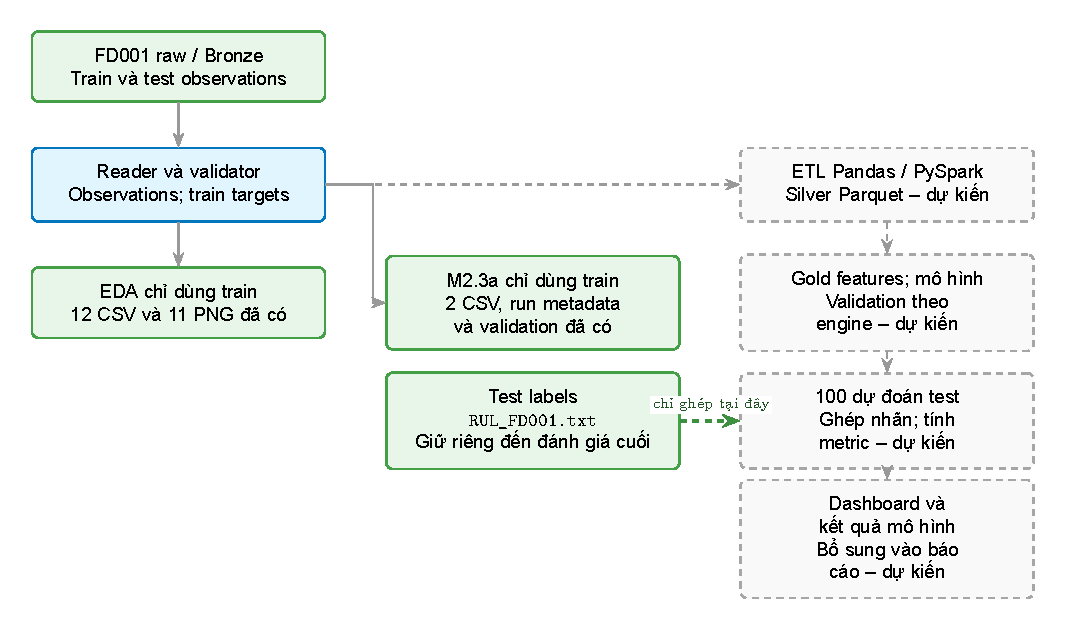
\includegraphics[width=0.98\linewidth]{figures/pipeline.pdf}
\caption[Luồng dữ liệu và trạng thái triển khai]{Luồng dữ liệu: đường liền thể
hiện nhánh đã hiện thực hóa hoặc đã có artifact; đường và khung nét đứt thể hiện
phần dự kiến. Nhãn test được vẽ như side input tách riêng và chỉ ghép vào bước
đánh giá cuối.}
\label{fig:pipeline}
\end{figure}

Bronze giữ dữ liệu nguồn để truy vết. Silver lưu observations đã gán kiểu dữ
liệu và train targets trong Parquet; Gold M3.1 lưu engine summary trong
Parquet/SQLite để kiểm tra boundary và truy vấn cục bộ. Gold M3.2 lưu rolling
features trong Parquet, tách khỏi bước fit scaler hoặc mô hình. Cách tách lớp
giúp phân biệt dữ liệu gốc với dữ liệu suy ra và xác định bước gây mất hoặc
nhân bản dòng.
Pandas là reference implementation; PySpark tái hiện ba boundary và parity
checker đã xác nhận ba bảng khớp với sai khác lớn nhất bằng 0 trong lần chạy
local có JRE. Chưa có bằng chứng để kết luận công cụ nào nhanh hơn.

FD001 có dung lượng nhỏ. Benchmark M3.1 ở mức $1\times$, $10\times$ và
$100\times$ chỉ đánh giá chi phí tạo engine summary; bản nhân dữ liệu đổi engine
ID và tách khỏi phân tích khoa học. Việc nhân bản quan sát không tạo thêm động
cơ độc lập để huấn luyện hoặc thu hẹp khoảng tin cậy.

\subsection{EDA theo đơn vị động cơ}
EDA chỉ sử dụng train để tìm hiểu dữ liệu mà không dựa vào test khi quyết định
phương pháp. Phân phối tuổi thọ tính mỗi động cơ một lần. Ngược lại, histogram
RUL theo quan sát cho động cơ sống lâu nhiều quan sát hơn. Hai cách tổng hợp trả
lời hai câu hỏi khác nhau và không được diễn giải thay thế nhau.

Correlation giữa sensor và RUL được tính bằng Spearman riêng trong từng động
cơ, sau đó tóm tắt phân phối giữa các động cơ. Lựa chọn này khảo sát liên hệ đơn
điệu và tránh để số dòng của một động cơ quyết định trực tiếp trọng số trong
bảng tổng hợp correlation. Tuy vậy, dependence theo thời gian vẫn tồn tại;
correlation mô tả chưa chứng minh quan hệ nhân quả hoặc hiệu quả dự đoán ngoài
mẫu.

Sensor hằng có correlation không xác định, được giữ dưới dạng NaN thay vì gán
0. Ba động cơ minh họa được chọn gần các tứ phân vị tuổi thọ; nếu bằng khoảng
cách, chọn ID nhỏ hơn. Quy tắc này dựa trên tuổi thọ, không dựa trên quỹ đạo
sensor có hình dạng dễ quan sát. Quỹ đạo hiện có biểu diễn giá trị gốc theo
cycle, không smooth; mỗi ô dùng thang đo riêng. Ba động cơ này không đại diện
thống kê. Tuổi thọ đầy đủ chỉ dùng cho phân tích hồi cứu sau khi đã quan sát cả
chuỗi, không được dùng làm feature dự đoán tại cycle hiện tại.


\subsection{Đặc trưng từ window M3.2}
Biểu diễn chính đã triển khai là trailing window (cửa sổ chỉ chứa hiện tại và
quá khứ) dài 30 cycles. Ví dụ, dự đoán tại cycle 170 dùng các cycle 141--170
của cùng động cơ. Mỗi output row khóa bởi \texttt{(split, engine\_id, cycle)},
trong đó \texttt{cycle} là cycle cuối của window. Transformer từ chối engine có
ít hơn 30 cycles; không padding, không impute và không rút ngắn window.

M3.2 giữ đủ 21 sensors trong artifact để chưa thực hiện feature selection trên
toàn bộ train. Với mỗi sensor, pipeline tạo sáu đặc trưng theo mẫu
\texttt{<sensor>\_\_<stat>}: giá trị cuối, mean, sample standard deviation
(\texttt{ddof=1}), min, max và linear slope theo vị trí 1--30 trong window. Nếu
một sensor bằng đúng số cycle trong window 1--30 thì các feature tương ứng là
\texttt{last=30}, \texttt{mean=15,5}, \texttt{min=1}, \texttt{max=30} và
\texttt{slope=1}. Sample standard deviation dùng quy ước thống kê mẫu để nhất
quán với cách mô tả biến thiên trong EDA, nhưng quyết định này được ghi riêng
trong \filepath{outputs/features/run\_info.json} thay vì suy ngầm từ default.

Artifact hiện có 27.927 rows, gồm 17.731 train windows và 10.196 test windows.
Bước này không đọc \filepath{data/raw/RUL\_FD001.txt}, không join nhãn test,
không fit scaler, không chọn sensor và không huấn luyện mô hình. Các lựa chọn
phụ thuộc dữ liệu như loại sensor hằng, PCA hoặc scaler vẫn phải học trong
training fold ở mốc mô hình.

\subsection{Mô hình và đánh giá: phần dự kiến}
Naive baseline theo trung vị RUL cung cấp mốc so sánh khi không dùng tín hiệu
sensor. Ridge là baseline tuyến tính có regularization; HistGradientBoostingRegressor
là ứng viên phi tuyến. So sánh này nhằm đánh giá lợi ích của tín hiệu sensor so
với dự đoán đơn giản và mức cải thiện khi cho phép quan hệ phi tuyến. Chưa có
hyperparameter search hoặc kết quả để xếp hạng ba phương pháp.

Model selection dự kiến dùng GroupKFold 5-fold theo \texttt{engine\_id}. Các
window liền nhau của một động cơ có thể dùng chung phần lớn quan sát: hai window
141--170 và 142--171 dùng chung 29 cycles. Nếu chia ngẫu nhiên theo dòng, những
window gần như giống nhau có thể nằm ở cả train và validation, gây data leakage
(rò rỉ dữ liệu). Vì vậy, toàn bộ window của một động cơ phải thuộc cùng fold;
scaler, lựa chọn sensor và mô hình chỉ fit trên training fold.

Metric chọn mô hình dự kiến là mean engine-level MAE. Với $m$ động cơ validation
và $n_i$ dự đoán được đánh giá của động cơ $i$, đặt
\begin{equation}
\mathrm{MAE}_{\mathrm{engine}}=\frac{1}{m}\sum_{i=1}^{m}\left[\frac{1}{n_i}\sum_{t\in\mathcal E_i}|y_{i,t}-\widehat y_{i,t}|\right],
\end{equation}
trong đó $\mathcal E_i$ là tập cycle được protocol chọn để đánh giá. Cách lấy
trung bình này cho mỗi động cơ trọng số bằng nhau. Quy tắc chọn $\mathcal E_i$
trong cross-validation còn phải được cụ thể hóa và lưu cùng cấu hình trước khi
huấn luyện. RMSE và NASA asymmetric score dự kiến là metric phụ; chưa có số liệu
cho các metric này.

Sau khi chọn cấu hình bằng train/validation, mô hình được refit trên toàn train
và tạo một dự đoán cho mỗi động cơ test tại cycle cuối quan sát. Chỉ sau đó mới
ghép nhãn test để đánh giá cuối. Khoảng tin cậy dự kiến dùng bootstrap theo động
cơ nhằm giữ nguyên đơn vị chuỗi, thay vì giả định các window chồng lấn là mẫu độc
lập.

\subsection{Thống kê hiện có và ARIMA dự kiến}
M2.3a--M2.3b so sánh trung bình 30 cycles đầu và 30 cycles cuối trong cùng động cơ,
theo quyết định ngày 22/09/2026. Helper tạo cặp và các hàm suy luận theo sensor
đã được hiện thực hóa, kiểm tra bằng fixture và chỉ xử lý train. Notebook 02 đã
xuất bảng cặp, bảng suy luận, metadata, validation và hai hình panel tại
\filepath{outputs/statistics/}; bảng cặp có 2.100 dòng và bảng suy luận có 21
dòng. Mục~\ref{sec:stat-protocol} định nghĩa cặp, chiều chênh lệch, đầu ra,
giả định và cấu hình M2.0 đã chốt. Mục~\ref{sec:theory} trình bày cơ sở của
chênh lệch cặp trung bình, khoảng tin cậy bootstrap 95\%, Wilcoxon và
Benjamini--Hochberg FDR. Hình phân phối và effect size được tạo theo panel
riêng cho từng sensor, kèm diễn giải về sensor hằng, dấu chênh lệch và
heterogeneity giữa các engine. Kết quả M2.3a--M2.3b không phải feature
selection và không kết luận về hiệu quả dự đoán RUL.

ARIMA là phân tích phụ trên Health Index từ PCA được fit trong training fold.
ARIMA không áp dụng trực tiếp lên nhãn RUL train vì Công thức~\ref{eq:rul} tạo
một countdown tất định; dự báo lại countdown không chứng minh khả năng khai thác
tín hiệu sensor. Kế hoạch hiện tại chọn 10 động cơ validation đại diện, dùng
70\% đầu chuỗi để fit và 30\% cuối để đánh giá. Cách chọn động cơ cụ thể và
ARIMA order còn chưa triển khai. Kết quả sẽ cần ADF, Ljung--Box, forecast
MAE/RMSE và coverage của khoảng dự đoán 95\%.

\clearpage
\section{Protocol thống kê suy luận mốc 2}
\label{sec:stat-protocol}
\subsection{Mục tiêu, phạm vi và trạng thái quyết định}
Mục tiêu là đánh giá mức thay đổi của sensor giữa đầu và cuối vòng đời trong cùng engine trên tập train FD001. Ngày 22/09/2026 đã chốt dùng trung bình \textbf{30 cycles đầu và 30 cycles cuối}. Phân tích chỉ đọc train và dùng engine làm đơn vị ghép cặp. Đây là protocol trước khi chạy kiểm định, được viết sau EDA; các giả thuyết phát sinh từ EDA mang tính khám phá, không được mô tả là đã đăng ký trước khi xem dữ liệu.

Các phương pháp paired analysis, effect size, bootstrap 95\%, Wilcoxon khi phù hợp, Benjamini--Hochberg và seed 42 thuộc kế hoạch hiện có. Các lựa chọn tính toán mới ở mục cuối được ghi là đề xuất cần chốt trước triển khai. Chưa có p-value, khoảng tin cậy hoặc kết luận suy luận từ protocol này.

\subsection{Định nghĩa cặp đầu/cuối và ví dụ}
Với $x_{i,t,s}$ là giá trị sensor $s$ của engine $i$ ở cycle $t$, và $T_i$ là cycle cuối của train engine đó, đặt
\begin{align}
 E_{i,s}&=\frac1{30}\sum_{t=1}^{30}x_{i,t,s},&
 L_{i,s}&=\frac1{30}\sum_{t=T_i-29}^{T_i}x_{i,t,s},\\
 D_{i,s}&=L_{i,s}-E_{i,s}.&&
 \label{eq:paired-difference}
\end{align}
$D_{i,s}>0$ biểu thị mức trung bình cuối đời lớn hơn đầu đời. Mỗi engine đóng góp một cặp cho mỗi sensor, bất kể tuổi thọ. Hai đoạn phải đủ dữ liệu, liên tục và không chồng lấn. Tuổi thọ train nhỏ nhất đã ghi nhận là 128 cycles, nên độ dài hiện tại đáp ứng điều kiện này; bước triển khai vẫn phải kiểm tra lại input contract.

Ví dụ tính chỉ số: với engine có $T_i=200$, đoạn đầu là cycles 1--30 và đoạn cuối là cycles 171--200. Không nhầm đoạn cuối đời này với window 141--170 dùng dự đoán tại cycle 170. $T_i$ được biết khi phân tích hồi cứu train; không được dùng để xác định đặc trưng ở thời điểm dự đoán trên test.

Giữ độ dài bằng nhau giúp so sánh hai mức tín hiệu trên cùng số cycles. Tuy nhiên, 30 cycles chiếm tỷ lệ vòng đời khác nhau giữa các engine. Protocol này trả lời câu hỏi về hai đoạn có độ dài tuyệt đối cố định, không phải so sánh cùng phần trăm tuổi thọ và cũng không tự xác định chính xác thời điểm bắt đầu suy giảm.

\begin{figure}[H]
\centering
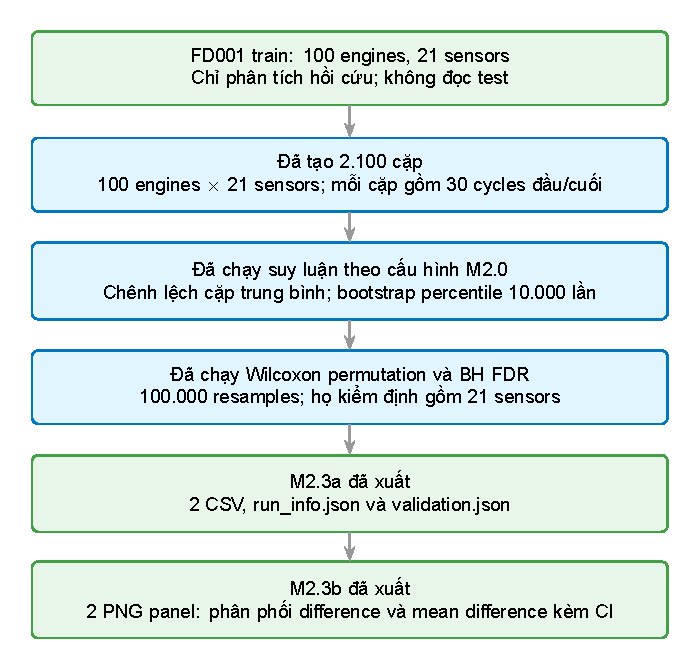
\includegraphics[width=0.91\linewidth]{figures/statistical-protocol.pdf}
\caption[Protocol thống kê đầu/cuối vòng đời]{Thiết kế phân tích mốc 2; chỉ bước chọn hai đoạn 30 cycles và các nguyên tắc đã nêu được chốt. Các phép tính suy luận chưa chạy, cấu hình chi tiết còn cần chốt.}
\label{fig:stat-protocol}
\end{figure}

\subsection{Đại lượng cần báo cáo và điều kiện diễn giải}
Bảng kết quả dự kiến giữ đủ 21 sensors, không chọn danh sách từ thứ hạng correlation của EDA. Ba operational settings không được gộp vào cùng họ giả thuyết sensor. Bảng cần có số cặp hợp lệ, số chênh lệch bằng 0, mức thay đổi, khoảng tin cậy, thống kê kiểm định, p-value gốc, p-value hiệu chỉnh và trạng thái có thể kiểm định.

Đề xuất dùng mean paired difference $\widehat\Delta_s=m^{-1}\sum_i D_{i,s}$ làm effect size theo đơn vị gốc, kèm median và phân phối $D_{i,s}$. Đây là đại lượng mô tả độ lớn thay đổi, không phải effect size chuẩn hóa và không so sánh trực tiếp độ lớn giữa các sensor khác thang đo. Không gán đơn vị vật lý nếu nguồn chưa xác nhận. Bootstrap lấy mẫu lại các engine cùng cặp $E,L$ để tạo khoảng tin cậy 95\% cho $\widehat\Delta_s$~\cite{scipyBootstrap}. Số lần lấy mẫu và phương pháp dựng khoảng còn ở mức đề xuất bên dưới.

Wilcoxon hai phía xét phân phối chênh lệch đối xứng quanh 0, với các cặp độc lập giữa engine~\cite{scipyWilcoxon}. Cần xem phân phối chênh lệch và ghi giới hạn đối xứng; bootstrap của mean không thay thế giả định này. Sensor hằng hoặc toàn bộ $D_{i,s}=0$ vẫn phải xuất hiện trong bảng dưới trạng thái không có biến thiên quan sát được. Không biến p-value không xác định thành 0 và không tự kết luận rằng sensor có giá trị dự đoán bằng 0.

Benjamini--Hochberg áp dụng cho một họ kiểm định đã xác định trước~\cite{benjamini1995fdr}. Đề xuất giữ họ gồm 21 sensors, dùng giá trị 1 chỉ trong vector hiệu chỉnh cho trường hợp không kiểm định được, đồng thời giữ p-value gốc là không áp dụng và ghi rõ trạng thái trong bảng. Quy ước này tránh thu nhỏ họ giả thuyết theo kết quả thuận lợi; nó không sửa được p-value thiếu hợp lệ hoặc bảo đảm FDR dưới mọi dạng phụ thuộc giữa sensors. Các khoảng tin cậy bootstrap riêng lẻ không phải simultaneous intervals.

\subsection{Cấu hình đề xuất cần chốt trước triển khai}
Các giá trị sau là đề xuất cụ thể để lượt triển khai có thể quyết định và ghi lại trước khi tính kết quả; chúng chưa phải cấu hình đã chạy hoặc quyết định do default thư viện tạo ra.
\begin{itemize}
\item Effect size chính: mean paired difference; kèm median để nhìn độ nhạy với phân phối lệch. Chưa bổ sung effect size chuẩn hóa nếu chưa có câu hỏi cần so sánh giữa sensors.
\item Bootstrap: 10.000 lần lấy mẫu lại 100 engines có hoàn lại, seed 42; đề xuất percentile interval tại các quantile 2,5\% và 97,5\%. Cần ghi rõ giới hạn độ bao phủ hữu hạn; không mặc định tương đương BCa. Trường hợp phân phối bootstrap suy biến phải gắn nhãn, không diễn giải khoảng bằng 0 là chắc chắn tuyệt đối.
\item Wilcoxon: hai phía; đề xuất bỏ zero differences theo quy ước \texttt{wilcox}, average ranks cho ties và phương pháp permutation khi cần xử lý ties/zeros. Số phép hoán vị và quy tắc làm tròn theo độ phân giải raw cần được cố định, kiểm tra bằng ví dụ tính tay trước khi chạy toàn bộ.
\item FDR: đề xuất $q=0{,}05$ trên họ 21 sensors như mô tả trên. Chưa tự thêm kiểm định thay thế hoặc điều chỉnh phương pháp dựa vào p-value vừa quan sát.
\end{itemize}

Phải chốt các mục còn mở này trước khi chạy mốc 2. Nếu dùng phương án khác, cập nhật protocol, lý do và thời điểm thay đổi trước khi tạo bảng kết quả; không trình bày lựa chọn mới như đã xác định từ đầu.

\subsection{Đầu ra và điều kiện nghiệm thu}
Đầu ra dự kiến gồm bảng cặp theo engine/sensor, bảng thống kê theo sensor, hình phân phối chênh lệch và effect size kèm khoảng tin cậy, cùng metadata ghi cấu hình và phiên bản. Không tạo artifact rỗng để thay kết quả chưa chạy.

Kiểm tra phải bao gồm chỉ số 30 cycles đúng trong từng engine, không chồng đoạn, ghép cặp một--một, ví dụ tính tay và trường hợp hằng/ties/zeros. Bootstrap phải lấy mẫu theo engine và giữ cặp; FDR cần được kiểm tra trên một vector p-value nhỏ có đáp án biết trước. Chạy lại với cùng input và seed phải tái lập kết quả; raw và EDA gốc giữ nguyên. Khi có kết quả mới cập nhật phần kết quả, nhật ký và bằng chứng kiểm tra.

Kết luận thống kê chỉ áp dụng cho thay đổi trên train mô phỏng theo protocol này. Phát hiện thay đổi không chứng minh quan hệ nhân quả hoặc hiệu quả dự đoán ngoài mẫu. Lựa chọn sensor cho mô hình vẫn phải học trong training fold; không dùng danh sách có ý nghĩa thống kê trên toàn train để chọn feature trước cross-validation.

\clearpage
\section{Kết quả và diễn giải}

\subsection{Kiểm tra dữ liệu}
Validation đạt cho observations train, nhãn RUL train và observations test. Tập
train có 20.631 dòng, tập test có 13.096 dòng; mỗi tập gồm 100 engine. Một trăm
test labels hợp lệ về cấu trúc nhưng được giữ tách khỏi EDA và suy luận trên
train. Các kiểm tra schema, khóa duy nhất, kiểu số hữu hạn và cycle liên tục đều
đạt.

\subsection{ETL Silver/Gold và benchmark}
Pipeline Pandas và PySpark đọc dữ liệu sau khi kiểm tra data contract. Silver gồm
33.727 observations train/test và 20.631 train targets. Gold gồm 200 dòng engine
summary trong Parquet và bảng truy vấn tương ứng trong SQLite. Các bảng được đọc
lại sau khi ghi.

\begin{table}[H]
\centering
\caption[Benchmark Pandas tạo engine summary]{Benchmark tạo engine summary trên
observations nhân bản trong bộ nhớ; dữ liệu nhân bản không dùng để huấn luyện.}
\label{tab:etl-benchmark}
\begin{tabular}{rrrrr}
\toprule Scale & Input rows & Engine rows & Cold (s) & Warm (s)\\\midrule
1$\times$ & 33.727 & 200 & 0,0195 & 0,0196\\
10$\times$ & 337.270 & 2.000 & 0,1589 & 0,1474\\
100$\times$ & 3.372.700 & 20.000 & 1,6752 & 1,6732\\
\bottomrule
\end{tabular}
\end{table}

Benchmark đo chi phí của phép tổng hợp cục bộ, không phải bằng chứng về xử lý
phân tán. Pandas và PySpark khớp schema, khóa, số dòng và giá trị số cho ba bảng
Silver/Gold; sai khác tuyệt đối lớn nhất đều bằng 0,0.

\subsection{Rolling features}
Rolling features dài 30 cycles gồm 17.731 train windows và 10.196 test windows,
tổng cộng 27.927 dòng. Mỗi dòng có khóa \texttt{(split, engine\_id, cycle)} và
126 feature columns cho 21 sensor, gồm \texttt{last}, \texttt{mean}, sample
\texttt{std}, \texttt{min}, \texttt{max} và \texttt{slope}. Test labels không
được ghép trong bước này.

\begin{table}[H]
\centering
\caption[Rolling features theo split]{Số rolling windows theo split.}
\label{tab:rolling-features}
\begin{tabular}{lrr}
\toprule Split & Engines & Rolling windows\\\midrule
Train & 100 & 17.731\\
Test & 100 & 10.196\\
Tổng & 200 & 27.927\\\bottomrule
\end{tabular}
\end{table}

Validator kiểm tra schema, khóa duy nhất, thứ tự canonical, số hữu hạn và đủ
trailing window trong từng engine. Tests tính tay xác nhận sample standard
deviation, slope, không dùng tương lai và không nối hai engine.

\subsection{Tuổi thọ động cơ trên train}
\begin{table}[H]
\centering
\caption[Thống kê tuổi thọ của 100 động cơ train]{Thống kê tuổi thọ, đơn vị
cycle.}
\label{tab:lifetime}
\begin{tabular}{lr@{\qquad}lr}
\toprule Thống kê & Giá trị & Thống kê & Giá trị\\\midrule
Trung bình & 206,31 & Độ lệch chuẩn mẫu & 46,34\\
Nhỏ nhất & 128 & Lớn nhất & 362\\
Tứ phân vị 25\% & 177 & Trung vị & 199\\
Tứ phân vị 75\% & 229,25 & Số động cơ & 100\\\bottomrule
\end{tabular}
\end{table}

\begin{figure}[H]
\centering
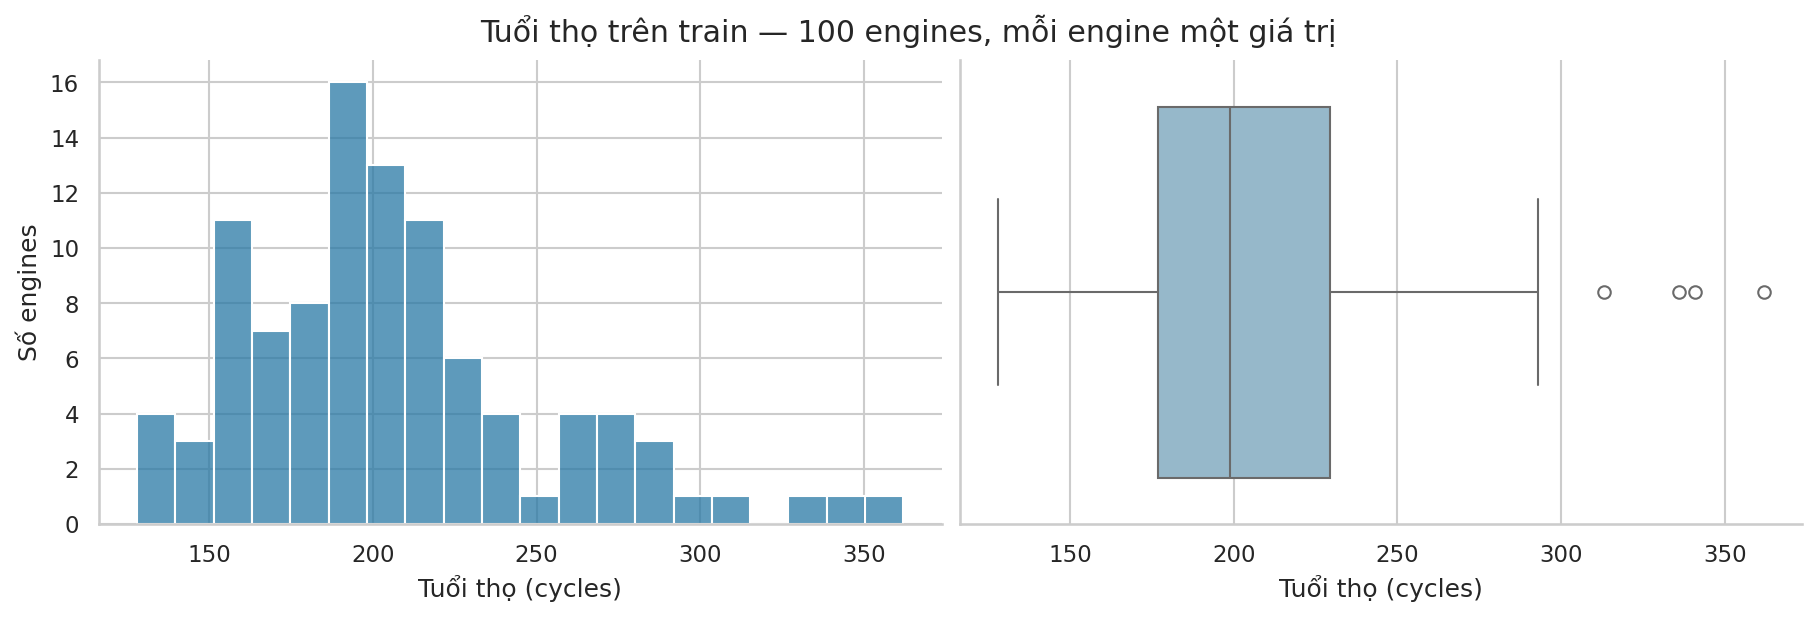
\includegraphics[width=0.9\linewidth]{../outputs/eda/figures/engine_lifetimes.png}
\caption[Phân phối tuổi thọ động cơ trên train]{Phân phối tuổi thọ train; mỗi
động cơ đóng góp một giá trị.}
\label{fig:life}
\end{figure}

Tuổi thọ dao động từ 128 đến 362 cycles; trung bình lớn hơn trung vị. Vì độ dài
chuỗi khác nhau, báo cáo phân biệt rõ tổng hợp theo observation và theo engine.
Các con số không được diễn giải thành tuổi thọ theo giờ hoặc ngày.

\subsection{Sensor hằng và correlation theo engine}
\begin{table}[H]
\centering
\caption[Correlation Spearman theo engine: các dòng minh họa]{Một số dòng minh
họa; bảng này không dùng để chọn sensor.}
\label{tab:correlation}
\begin{tabular}{lrrr}
\toprule Sensor & Động cơ xác định & Tương quan trung vị & Không xác định\\\midrule
1 & 0 & Không xác định & 100\\
6 & 62 & $-0{,}1264$ & 38\\
11 & 100 & $-0{,}8190$ & 0\\
12 & 100 & $0{,}8075$ & 0\\\bottomrule
\end{tabular}
\end{table}

Sensor 1, 5, 10, 16, 18 và 19 hằng trên train. Sensor 6 hằng trong 38/100
engine; correlation chỉ xác định trong 62 engine còn lại. Sensor 11 có tương
quan trung vị âm, còn sensor 12 có tương quan trung vị dương với RUL. Đây là
liên hệ mô tả trên train, không phải bằng chứng nhân quả hoặc hiệu quả ngoài mẫu.

\begin{figure}[H]
\centering
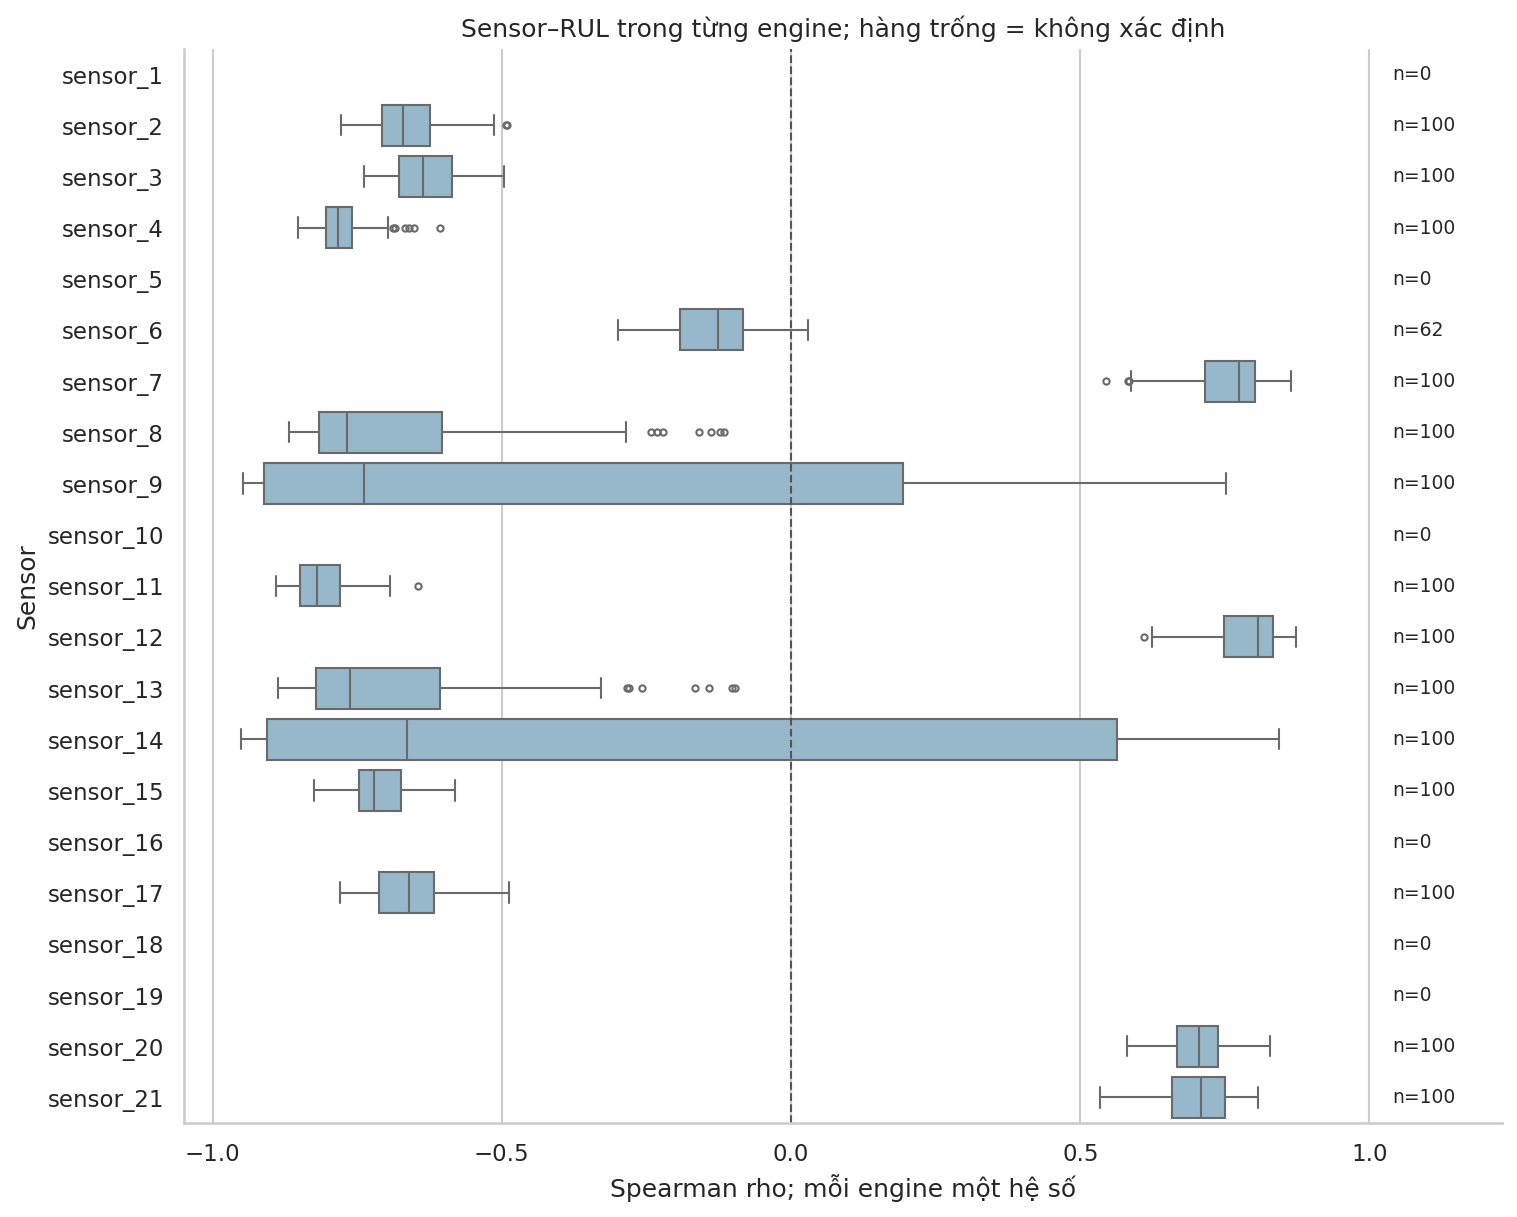
\includegraphics[width=\linewidth]{../outputs/eda/figures/sensor_rul_by_engine.png}
\caption[Phân phối correlation Spearman sensor--RUL theo động cơ]{Phân phối
correlation Spearman giữa các engine train. Sensor hằng được giữ là không xác
định.}
\label{fig:corr}
\end{figure}

\subsection{Suy luận đầu/cuối vòng đời trên train}
Bảng cặp gồm 2.100 dòng, tương ứng 100 engine train nhân 21 sensor. Mỗi dòng
dùng mean của 30 cycles đầu, mean của 30 cycles cuối và chênh lệch cuối trừ đầu.
Bảng suy luận giữ đủ 21 sensor.

Trong 21 sensor, sáu sensor có toàn bộ chênh lệch bằng 0:
\texttt{sensor\_1}, \texttt{sensor\_5}, \texttt{sensor\_10},
\texttt{sensor\_16}, \texttt{sensor\_18} và \texttt{sensor\_19}. Mười lăm
sensor còn lại kiểm định được; với cấu hình Wilcoxon permutation và
Benjamini--Hochberg trên họ 21 sensor, các p-value đã hiệu chỉnh đều xấp xỉ
0,000028.

\begin{table}[H]
\centering
\caption[Ví dụ kết quả suy luận sensor đầu/cuối]{Một số kết quả tiêu biểu. Giá
trị là chênh lệch cuối trừ đầu theo đơn vị gốc của từng sensor.}
\label{tab:sensor-inference}
\begin{tabular}{lrrl}
\toprule Sensor & Chênh lệch trung bình & Khoảng tin cậy bootstrap 95\% & Dấu chính\\\midrule
\texttt{sensor\_4} & 20,128097 & [19,402735; 20,865606] & Tăng\\
\texttt{sensor\_7} & -1,913527 & [-1,999307; -1,829684] & Giảm\\
\texttt{sensor\_11} & 0,613257 & [0,589017; 0,637944] & Tăng\\
\texttt{sensor\_12} & -1,627190 & [-1,704288; -1,552119] & Giảm\\
\texttt{sensor\_20} & -0,377007 & [-0,391534; -0,363173] & Giảm\\\bottomrule
\end{tabular}
\end{table}

\begin{figure}[H]
\centering
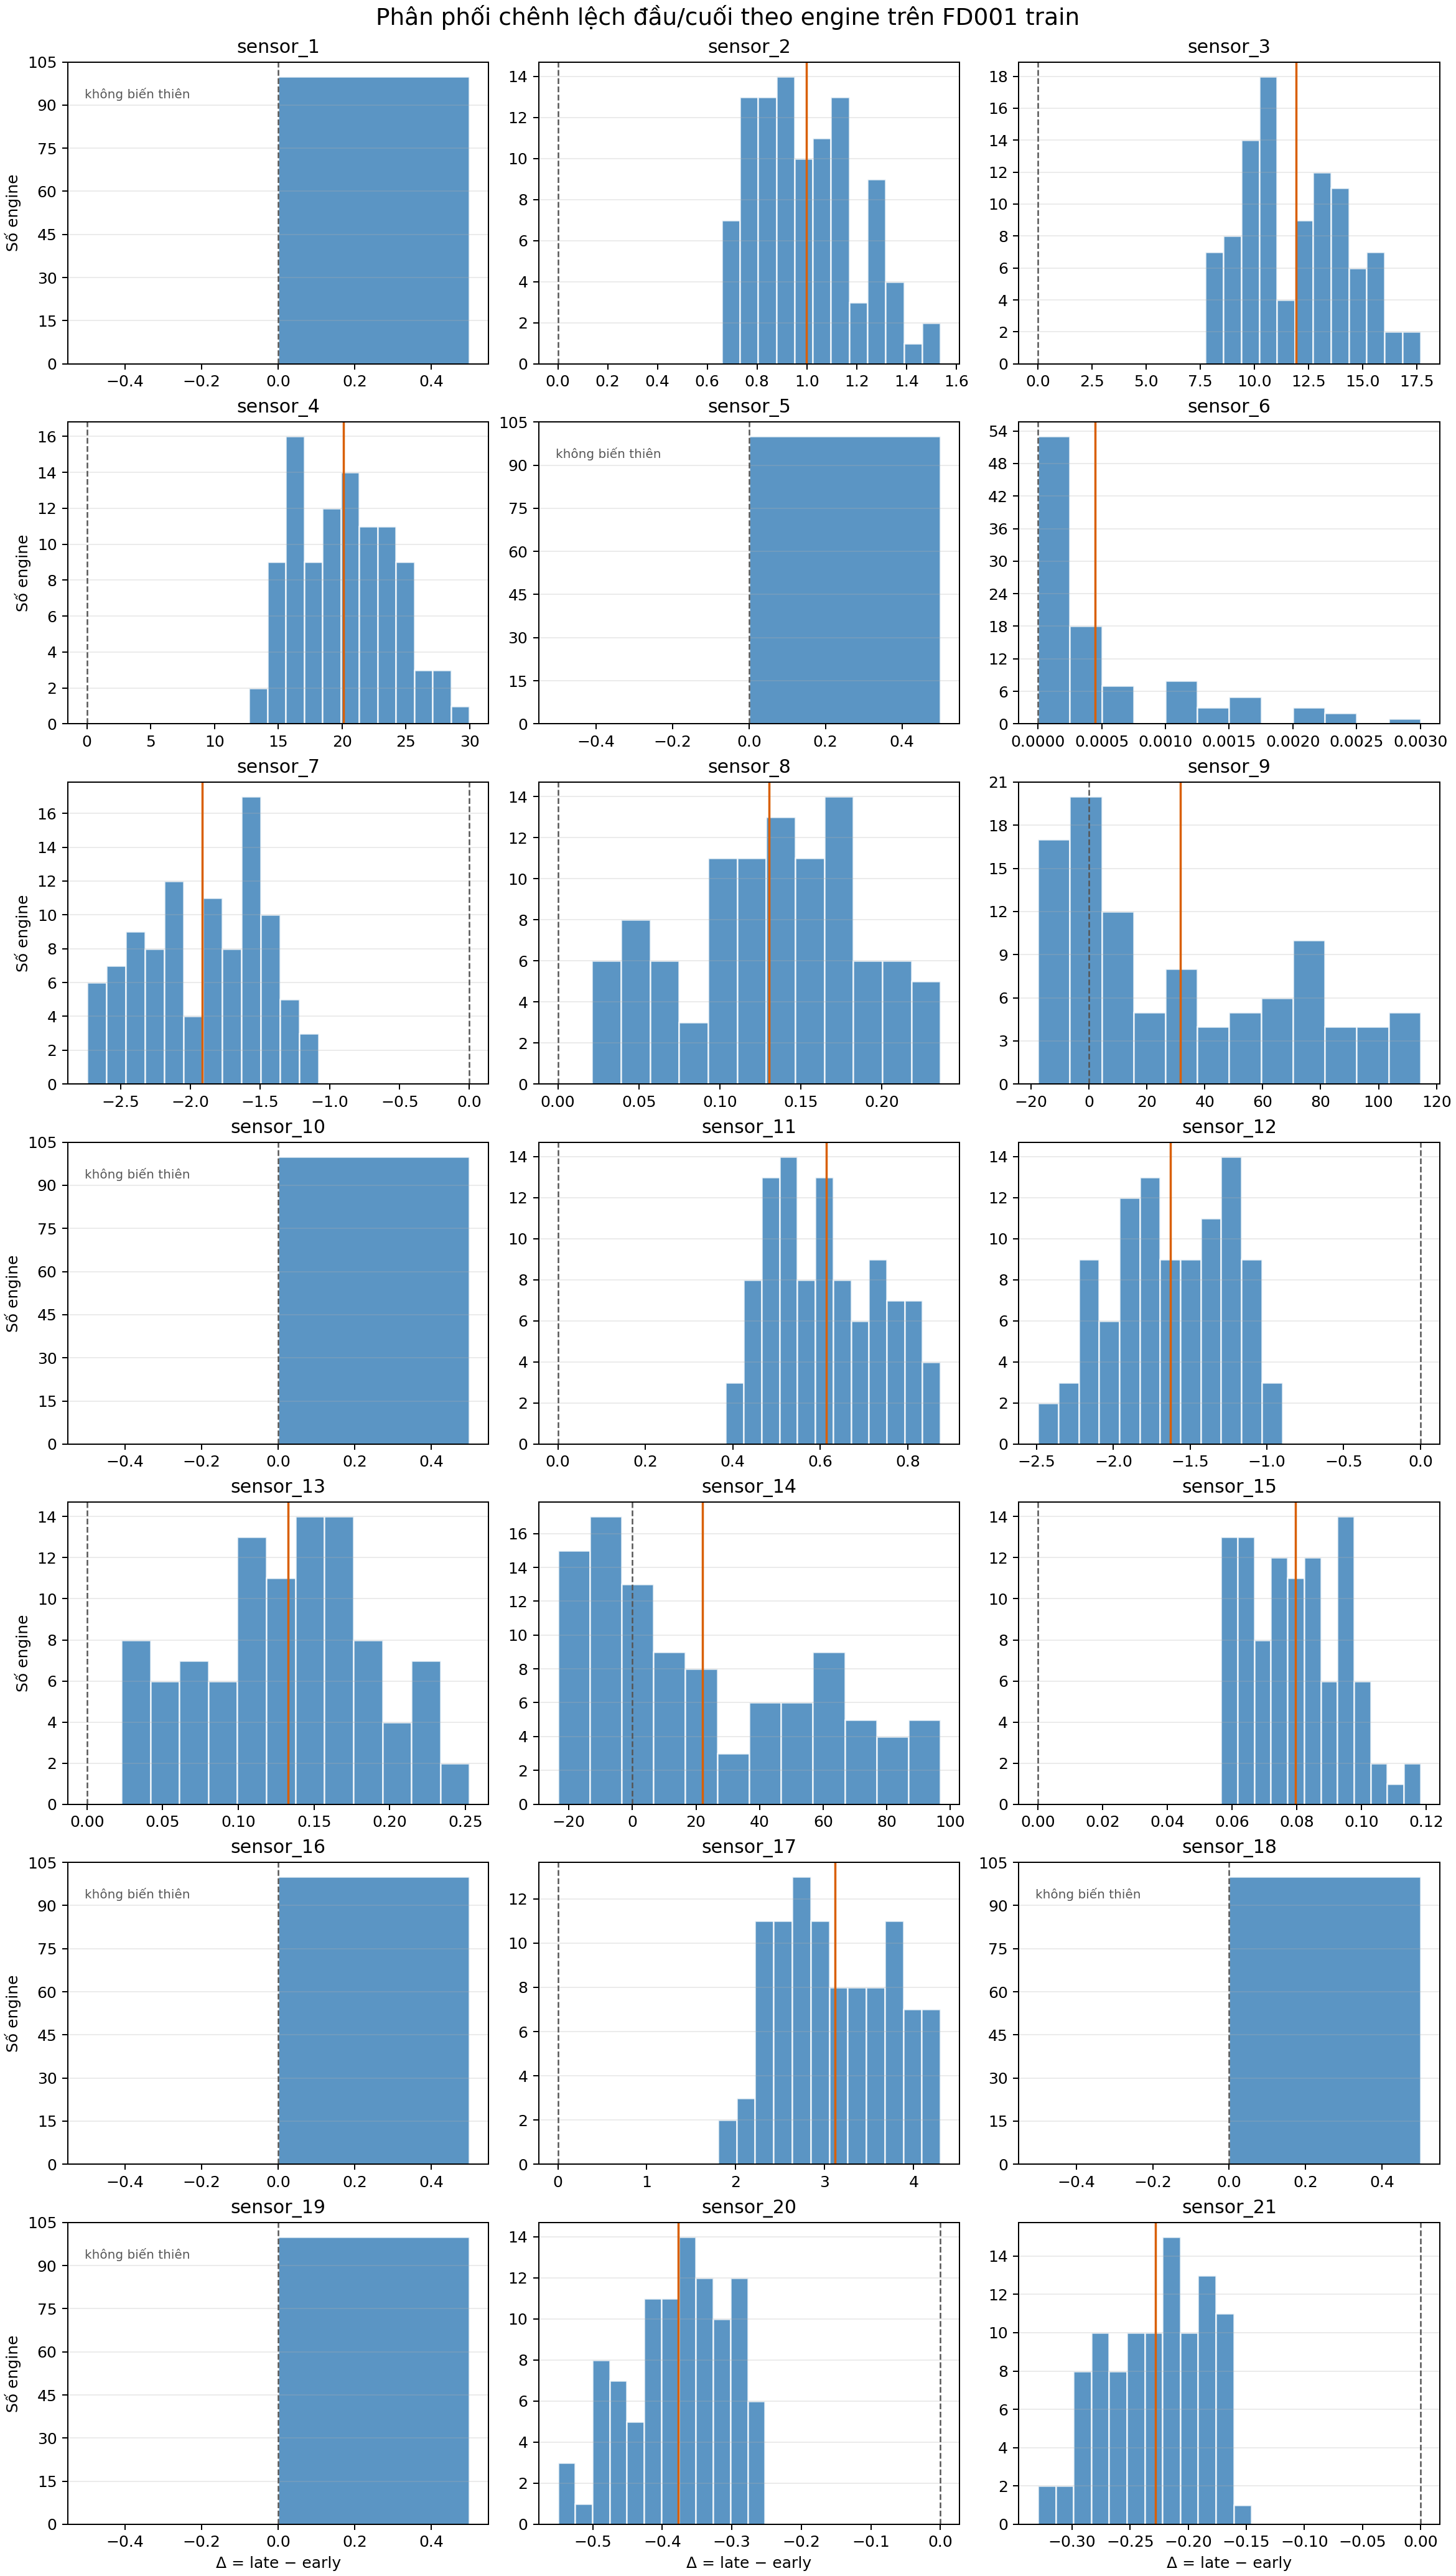
\includegraphics[width=0.86\linewidth,height=0.78\textheight,keepaspectratio]{../outputs/statistics/figures/difference_distributions.png}
\caption[Phân phối chênh lệch sensor đầu/cuối theo engine]{Phân phối chênh lệch
cuối trừ đầu của 100 engine cho từng sensor.}
\label{fig:statistics-distributions}
\end{figure}

\begin{figure}[H]
\centering
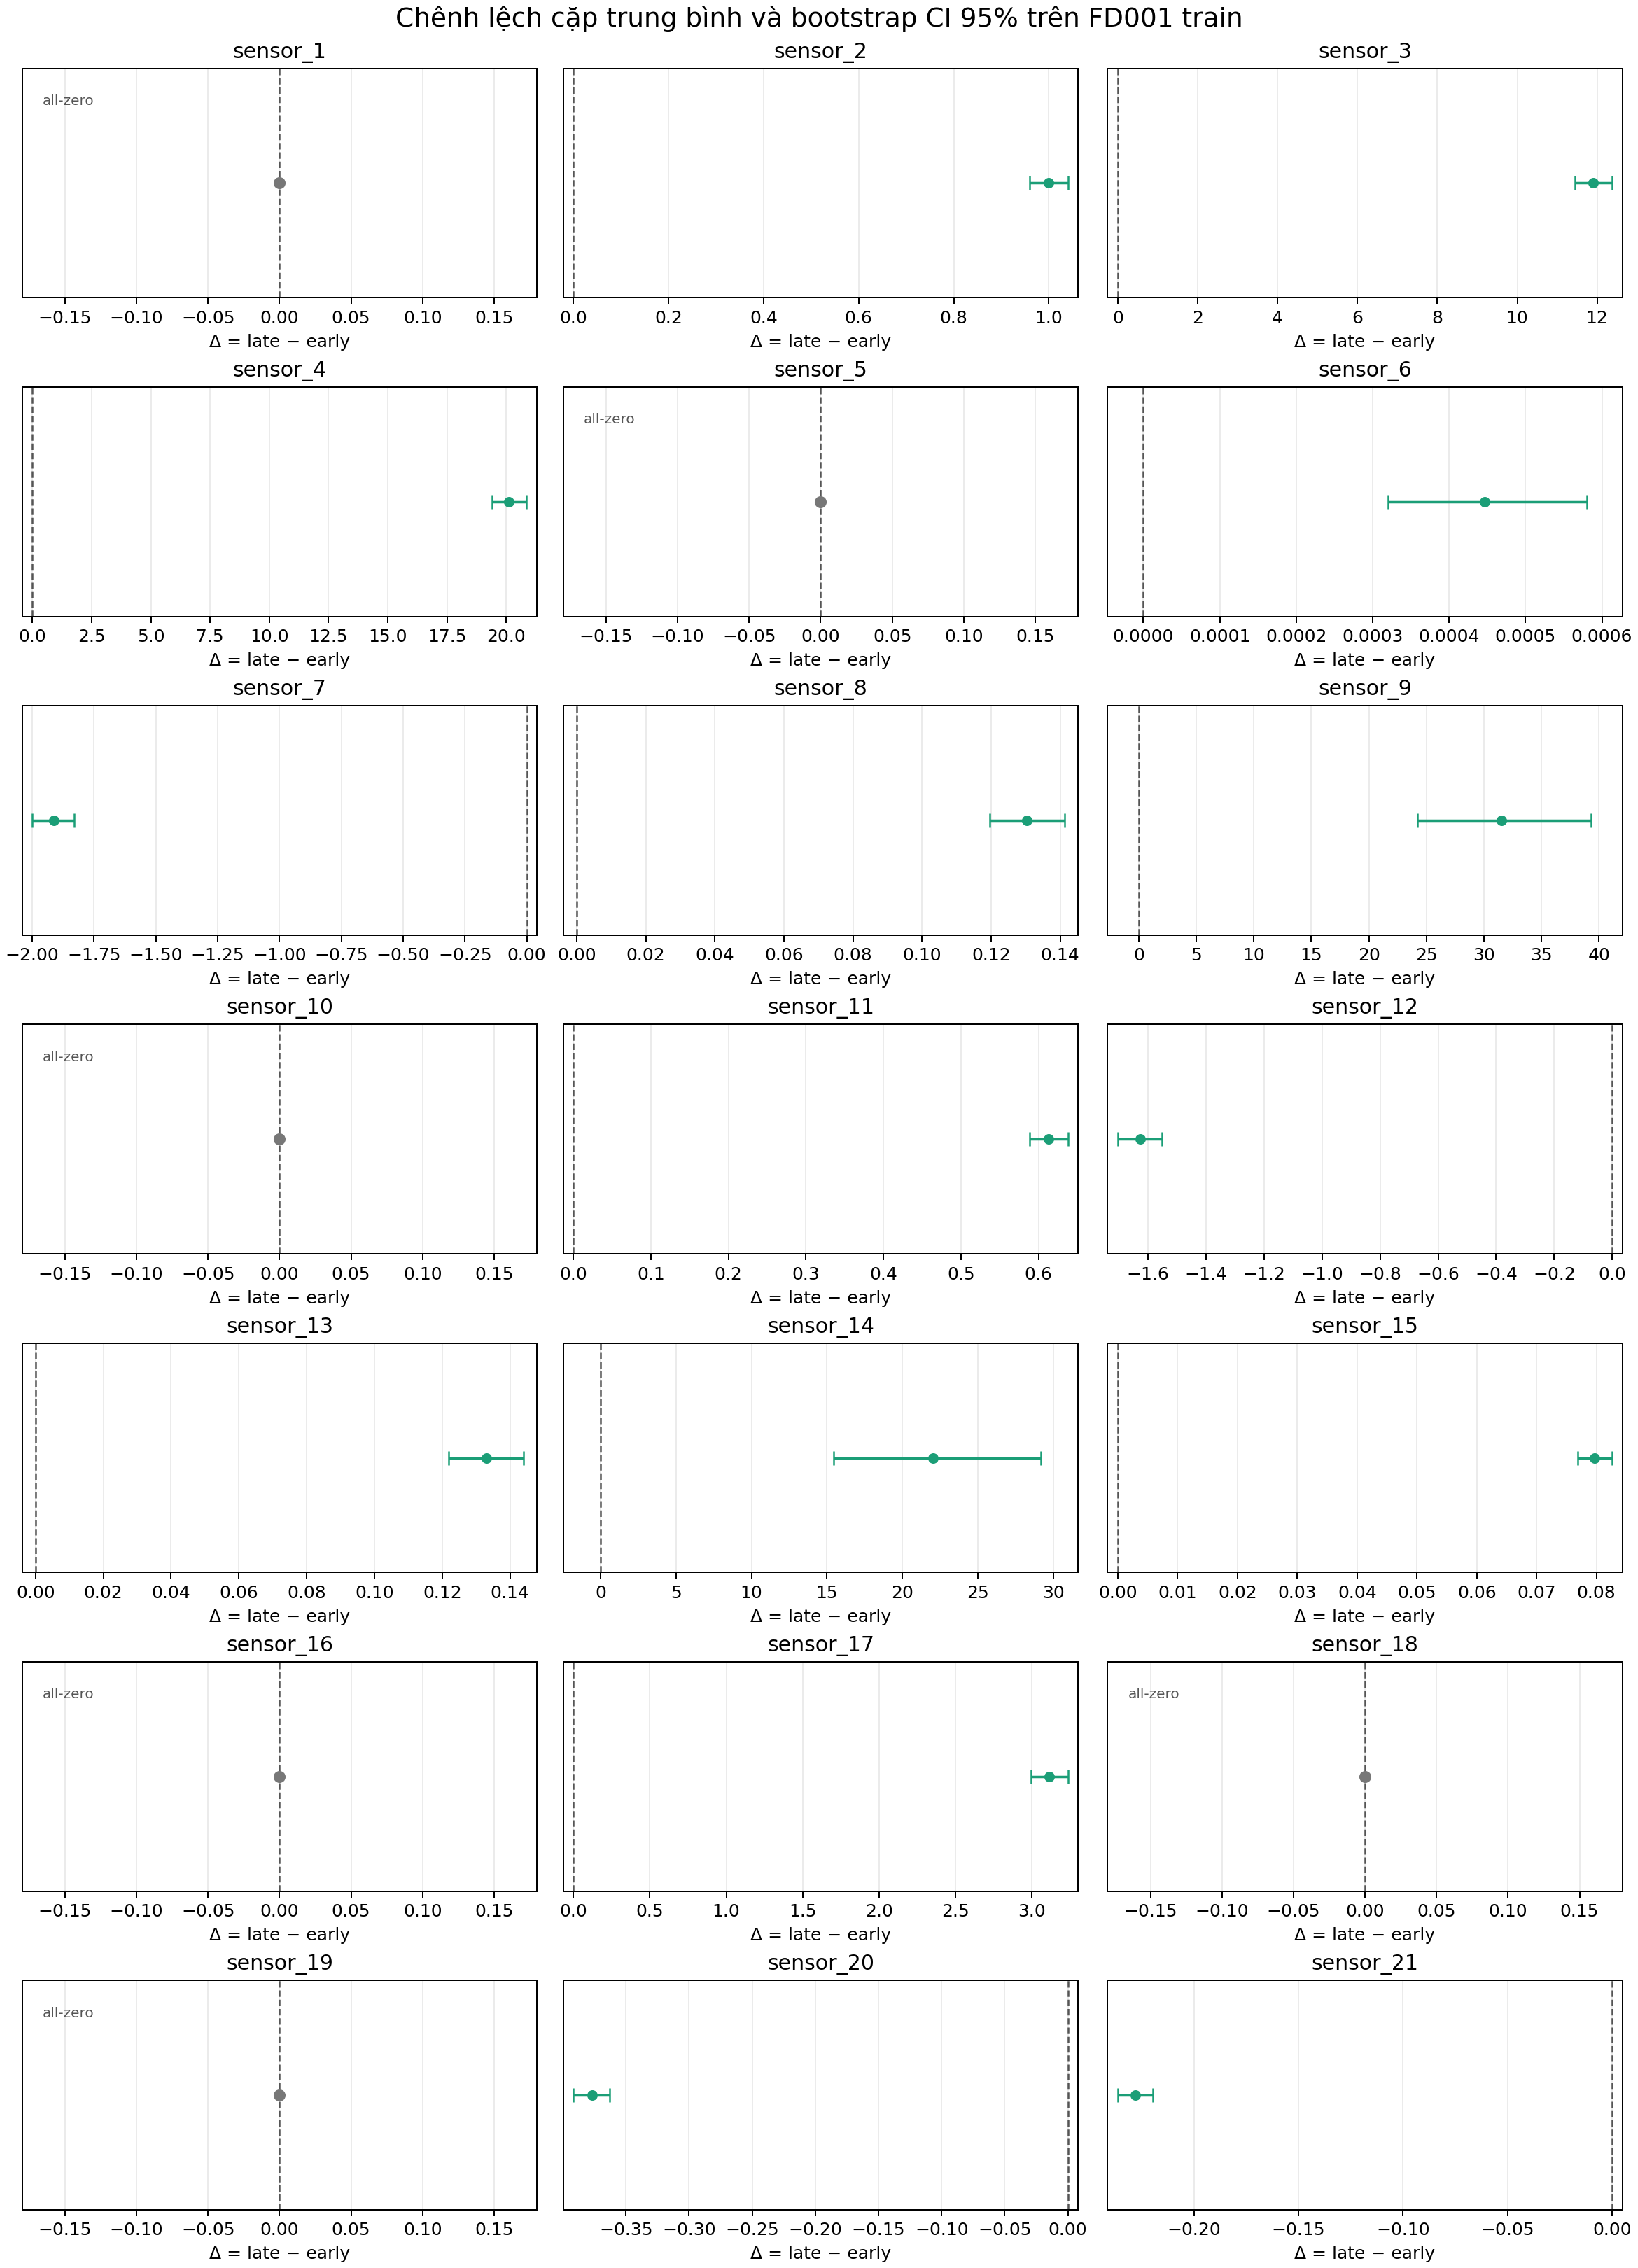
\includegraphics[width=0.86\linewidth,height=0.78\textheight,keepaspectratio]{../outputs/statistics/figures/effect_size_ci.png}
\caption[Chênh lệch cặp trung bình và khoảng tin cậy bootstrap]{Mean paired
difference và bootstrap CI 95\% theo từng sensor.}
\label{fig:statistics-effect-ci}
\end{figure}

Kết quả cho thấy nhiều sensor thay đổi có hệ thống giữa hai đoạn 30 cycles trên
train FD001 theo protocol đã chọn. Sensor 4 có chênh lệch trung bình khoảng
20,13, còn sensor 7 giảm khoảng 1,91; hai giá trị không được xếp hạng trực tiếp
vì khác thang đo. Sensor 6 có 47 chênh lệch dương và 53 chênh lệch bằng 0 nhưng
mean difference chỉ khoảng 0,00045; p-value nhỏ không đồng nghĩa thay đổi lớn.
Phân tích này không phải bằng chứng chọn feature hoặc utility dự đoán RUL ngoài
mẫu.

\clearpage
\section{Thảo luận}
\label{sec:discussion}

Mục này giải thích các kết quả ở Mục~\ref{sec:results}: sai số của mô hình RUL,
thời điểm cảnh báo, sự khác biệt giữa hai biểu diễn HGB126/HGB169 và khả năng
chuyển miền sang các subset khác. Các số liệu chẩn đoán dùng
trong mục này được tính lại từ artifact đã có bằng
\filepath{scripts/report_error_diagnostics.py}, không huấn luyện lại mô hình.

\subsection{Sai số của mô hình RUL đến từ đâu}
\label{sec:disc-error}
Bảng~\ref{tab:oof-by-rul} và Hình~\ref{fig:oof-pred-true} chia sai số OOF của
HGB126 trên train theo RUL thật. Mô
hình dự đoán tốt ở cuối vòng đời: MAE chỉ 3,67 cycles khi RUL thật không quá 30.
Sai số tăng dần khi RUL lớn hơn, và thay đổi hẳn tính chất khi RUL vượt khoảng
150 cycles. Ở vùng này, dự đoán trung bình gần như không đổi, quanh 145--147
cycles, bất kể RUL thật là 160 hay 300. Nói cách khác, mô hình đã tự học ra một
``trần'' khoảng 145 cycles, và mọi động cơ còn xa thời điểm hỏng đều bị dự đoán
gần mức đó.

\begin{table}[H]
\centering
\caption[Sai số OOF theo RUL]{Sai số OOF của HGB trên 17.731 window train, chia theo RUL thật.
Sai số có dấu bằng dự đoán trừ thật.}
\label{tab:oof-by-rul}
\small
\begin{tabular}{lrrrr}
\toprule
RUL thật (cycles) & Số window & MAE & Sai số có dấu trung bình & Dự đoán trung bình\\\midrule
0--30 & 3.100 & 3,67 & $+1{,}47$ & 16,47\\
31--60 & 3.000 & 10,68 & $+5{,}59$ & 51,09\\
61--90 & 3.000 & 20,85 & $+14{,}52$ & 90,02\\
91--125 & 3.392 & 22,81 & $+12{,}88$ & 120,61\\
126--150 & 1.999 & 20,82 & $-2{,}87$ & 134,73\\
151--200 & 2.226 & 30,25 & $-23{,}30$ & 147,16\\
201--361 & 1.014 & 91,29 & $-91{,}29$ & 145,36\\
\bottomrule
\end{tabular}
\end{table}

\begin{figure}[H]
\centering
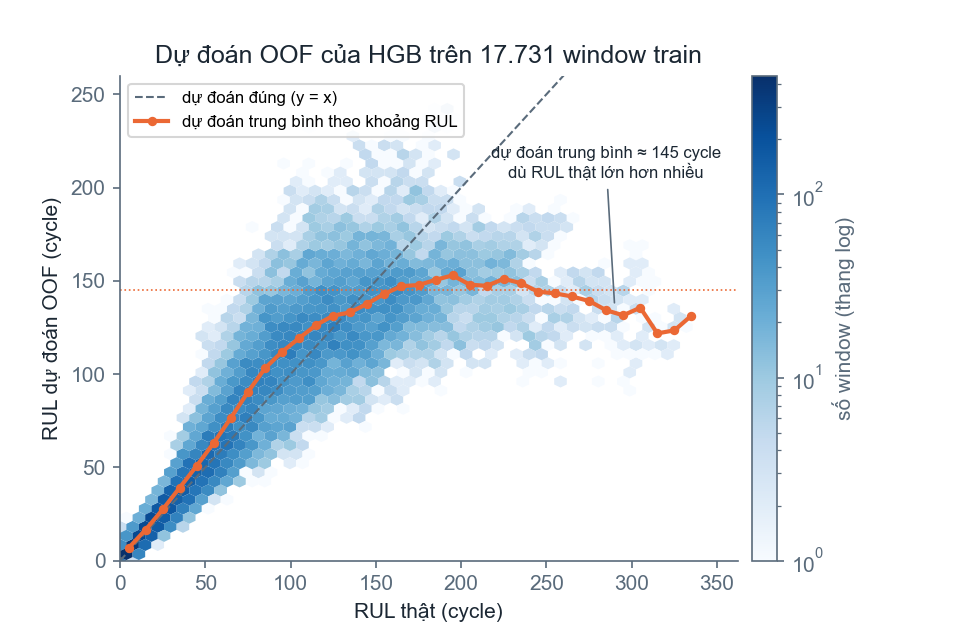
\includegraphics[width=0.6\linewidth]{../outputs/diagnostics/figures/oof_pred_vs_true.png}
\caption[RUL OOF so với thật]{RUL dự đoán OOF so với RUL thật. Đường cam là dự đoán trung bình theo
từng khoảng 10 cycles: bám sát đường chéo khi RUL nhỏ, nhưng dừng quanh 145 cycles
khi RUL thật lớn hơn khoảng 150.}
\label{fig:oof-pred-true}
\end{figure}

Hiện tượng này phù hợp với hình dạng của tín hiệu. Hình~\ref{fig:hi-trajectories}
cho thấy Health Index của các động cơ gần như đi ngang, chỉ dao động quanh một
mức, trong phần lớn vòng đời và chỉ giảm rõ ở giai đoạn cuối. Khi động cơ còn
khỏe, sensor chủ yếu phản ánh dao động đo và khác biệt ban đầu giữa các động cơ,
nên khó phân biệt một động cơ còn 160 cycles với một động cơ còn 300 cycles.
Kết quả này phù hợp với giả thuyết rằng biểu diễn hiện tại chứa ít tín hiệu phân
biệt RUL xa; dữ liệu hiện có chưa đủ để khẳng định một giới hạn thông tin cố định.
Nó cũng giải thích vì sao MAE cross-validation (20,21
cycles) cao hơn MAE test (15,35 cycles): 29,5\% số window train có RUL thật trên
125, trong khi RUL thật của test chỉ từ 7 đến 145.

\begin{figure}[H]
\centering
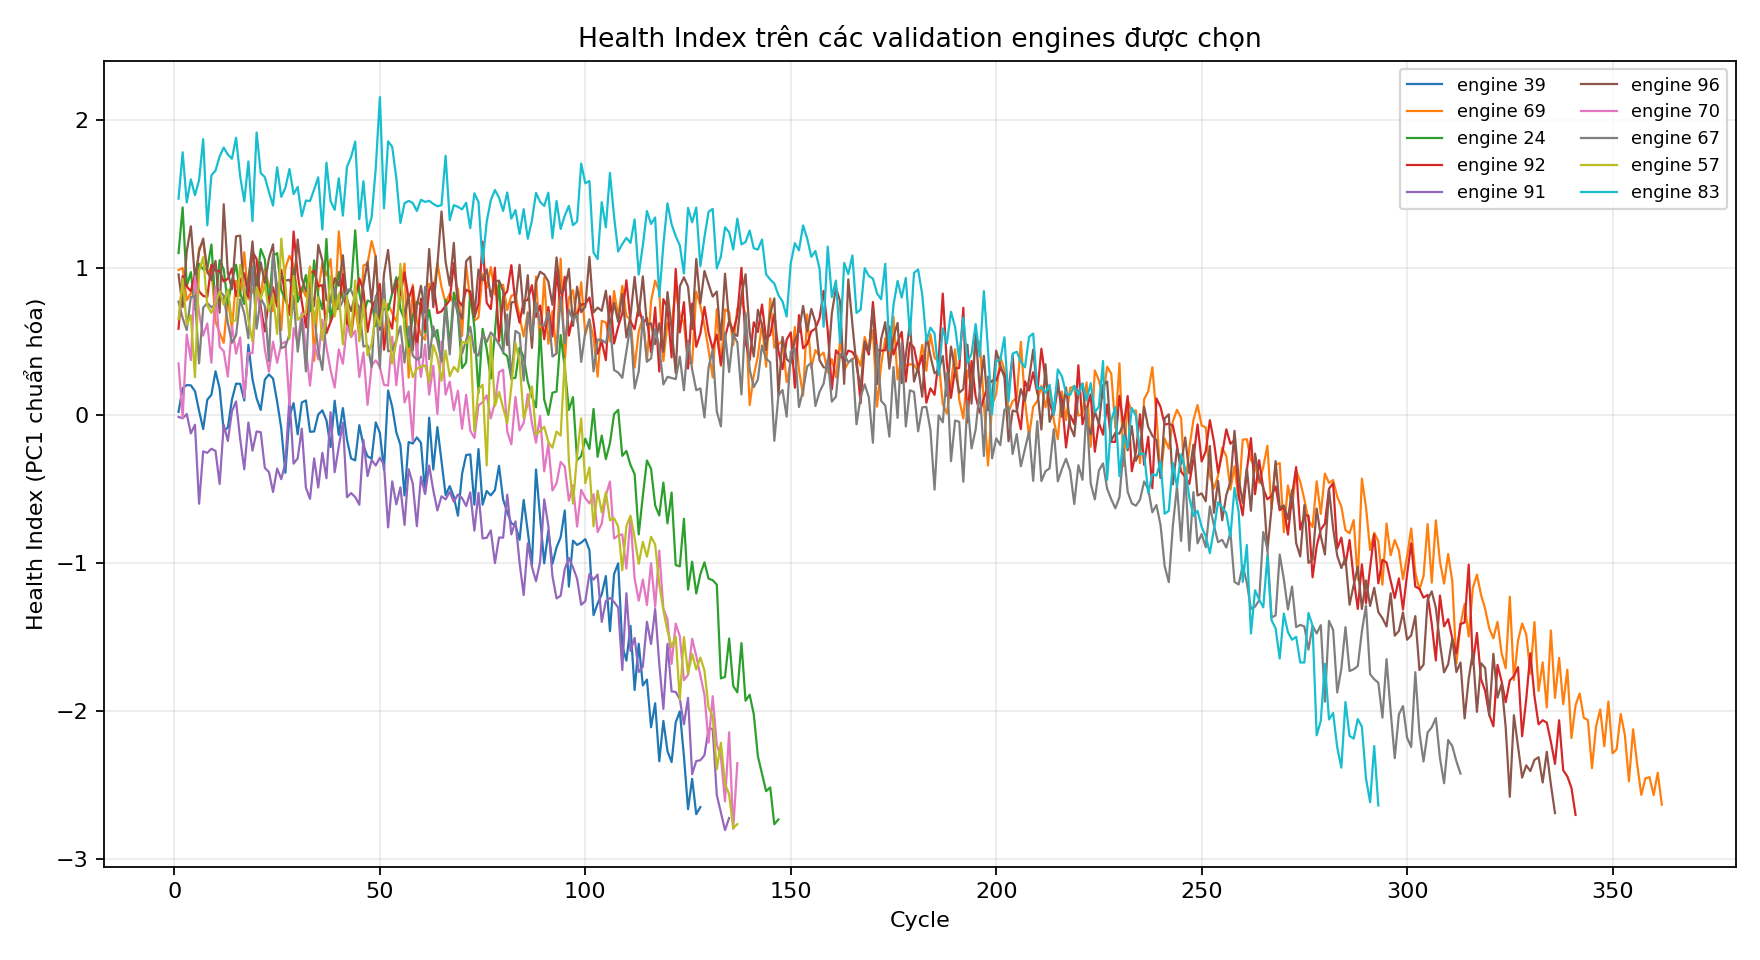
\includegraphics[width=0.6\linewidth]{../outputs/timeseries/figures/health_index_selected_engines.png}
\caption[Health Index của 10 động cơ]{Health Index theo cycle của 10 động cơ train được chọn ở Mục~\ref{sec:arima-method}.
Chỉ số gần như đi ngang ở phần lớn vòng đời và giảm rõ ở giai đoạn cuối.}
\label{fig:hi-trajectories}
\end{figure}

Ở vùng giữa (RUL 61--125), mô hình có xu hướng dự đoán cao hơn thật khoảng
13--15 cycles. Mười sai số lớn nhất trên test rơi vào các động cơ có RUL thật
77--137, phần lớn trùng với vùng này, và đều là dự đoán cao; riêng mười trường hợp
này chiếm 75,5\% NASA score. Như vậy, sai số test không phải ngẫu nhiên mà lặp lại
đúng xu hướng đã thấy trên OOF.

So với nghiên cứu liên quan, Li và cộng sự báo cáo RMSE 12,61 cycles trên FD001
với CNN khi cắt nhãn ở 125 cycles, và 13,32 cycles khi không cắt
nhãn~\cite{li2018rul}. RMSE của báo cáo là 20,54 cycles. Hai kết quả không so sánh
trực tiếp được, vì Li và cộng sự dùng 14 sensor, cách chuẩn hóa và mô hình khác.
Tuy vậy, khoảng cách khoảng 7 cycles so với cả phương án không cắt nhãn cho thấy
việc chỉ cắt nhãn có thể chưa đủ: sáu thống kê trên window 30 cycles có thể đã
làm mất một phần thông tin về hình dạng chuỗi mà CNN khai thác được.

\subsection{Vì sao gần một nửa cảnh báo bị trễ}
\label{sec:disc-warning}
Cảnh báo trễ không phân bố đều giữa các động cơ. 49 động cơ bị cảnh báo sau
ngưỡng có tuổi thọ trung bình 182,8 cycles, trong khi 44 động cơ được cảnh báo
trước ngưỡng có tuổi thọ trung bình 229,1 cycles. Hệ số tương quan giữa tuổi thọ
và độ lệch cảnh báo $\delta_i$ là $-0{,}56$: động cơ càng ngắn đời thì càng bị
cảnh báo muộn (Hình~\ref{fig:warning-lifetime}).

\begin{figure}[H]
\centering
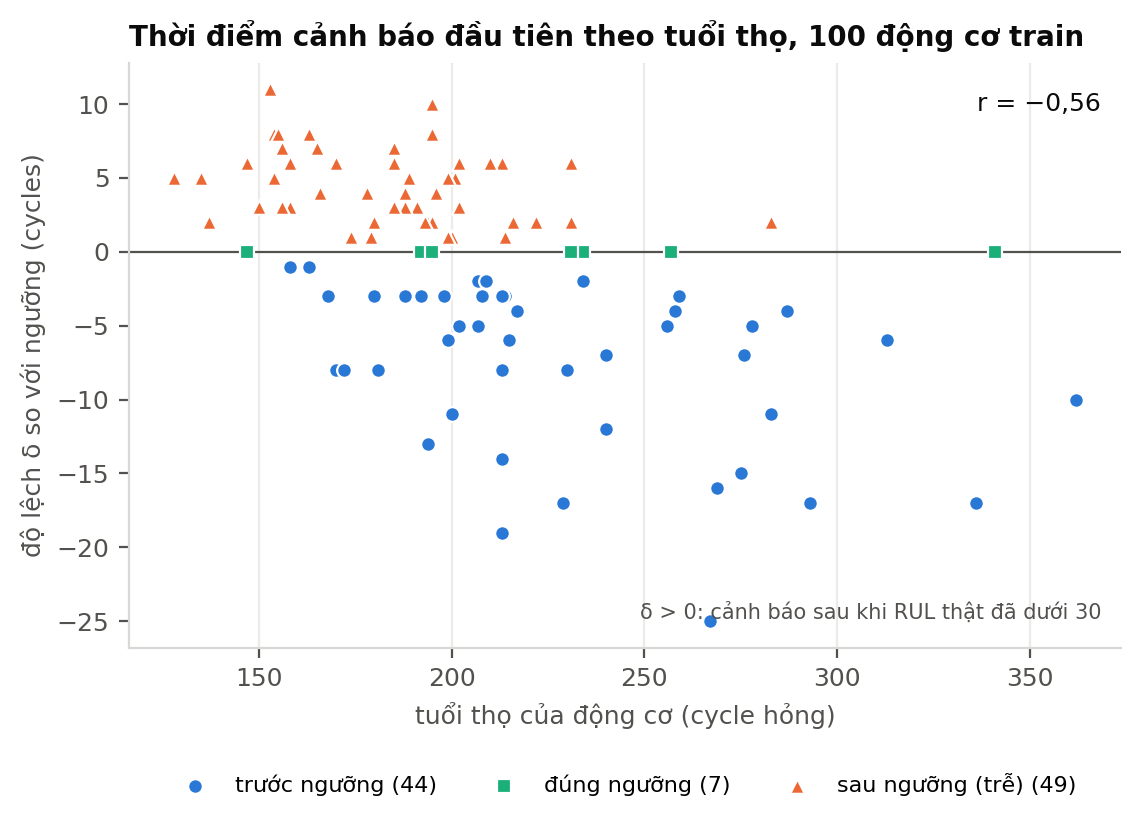
\includegraphics[width=0.62\linewidth]{../outputs/diagnostics/figures/warning_vs_lifetime.png}
\caption[Cảnh báo theo tuổi thọ]{Độ lệch của cảnh báo đầu tiên so với ngưỡng theo tuổi thọ của 100 động
cơ train. Cảnh báo trễ (tam giác cam) tập trung ở các động cơ hỏng trước khoảng
cycle 230.}
\label{fig:warning-lifetime}
\end{figure}

Một cách giải thích là mô hình học một quan hệ ``trung bình'' giữa mức sensor và
RUL. Động cơ ngắn đời suy giảm nhanh hơn trung bình, nên tại cùng một mức sensor,
RUL thật của chúng thấp hơn điều mô hình kỳ vọng. Kết quả là RUL dự đoán giảm
xuống dưới 30 muộn hơn thực tế. Điều này nhất quán với sai số dương ở vùng RUL
31--90 trong Bảng~\ref{tab:oof-by-rul}. Đặc trưng độ dốc trong window 30 cycles
lẽ ra phải phản ánh tốc độ suy giảm, nhưng trên 30 cycles, xu hướng thật có thể
bị dao động ngắn hạn che khuất. Phân tích trailing mean chỉ cho thấy biến động
được làm dịu trong mô tả tín hiệu; nó không chứng minh dữ liệu có nhiễu đo đã
biết hoặc rằng smoothing chắc chắn cải thiện RUL.

Từ góc độ ứng dụng, đây là loại lỗi nguy hiểm hơn cả: động cơ hỏng nhanh nhất lại
là động cơ nhận cảnh báo muộn nhất. Một ngưỡng cố định 30 cycles vì vậy chưa đủ.
Muốn bảo đảm lead time tối thiểu, ngưỡng cần có biên an toàn, hoặc mô hình cần
biết được tốc độ suy giảm riêng của từng động cơ. Cũng cần nhớ rằng các con số
cảnh báo được tính trên cùng tập OOF đã dùng để chọn mô hình, nên trên dữ liệu
mới, tỷ lệ cảnh báo trễ có thể còn cao hơn.

\subsection{Vì sao mô hình FD001 không chuyển được sang subset khác}
\label{sec:disc-transfer}
Bảng~\ref{tab:transfer-diagnostics} và Hình~\ref{fig:transfer-shift} cho thấy mô
hình FD001 thất bại theo hai kiểu khác nhau.

\begin{figure}[H]
\centering
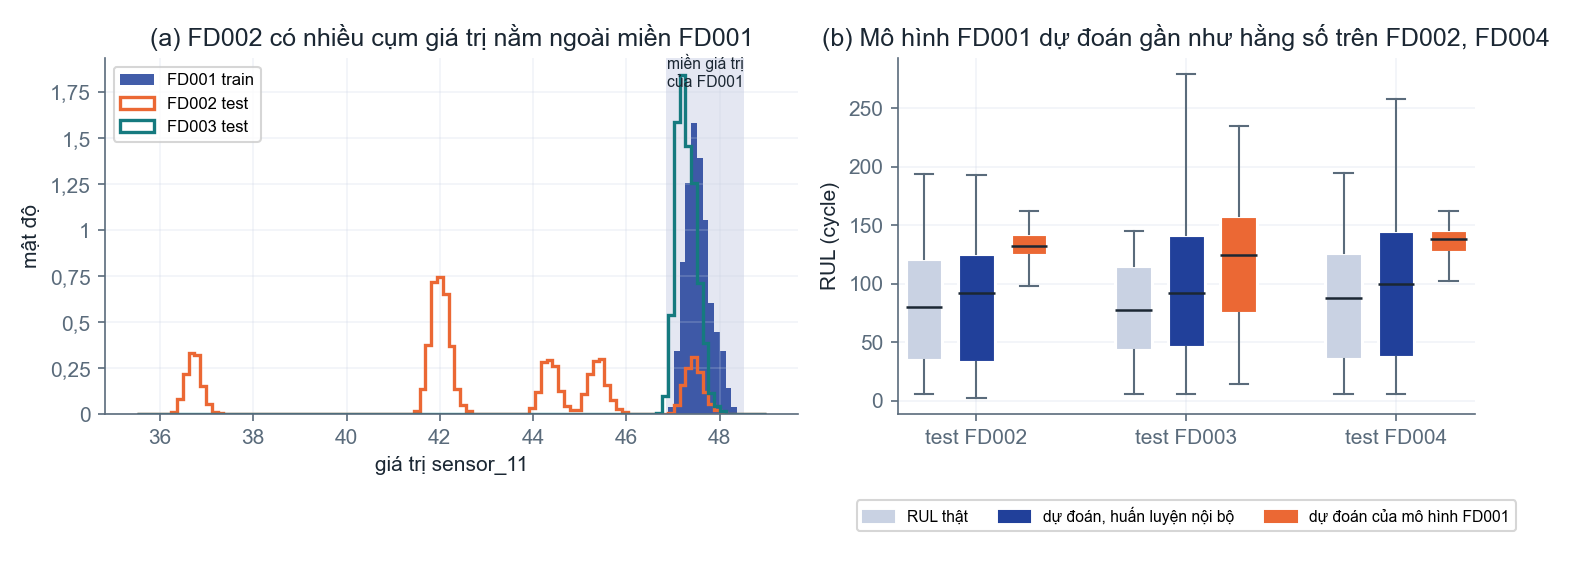
\includegraphics[width=\linewidth]{../outputs/diagnostics/figures/transfer_shift.png}
\caption[Dịch chuyển phân phối sensor]{(a) Phân phối \texttt{sensor\_11}: FD003 nằm trong miền giá trị của FD001,
còn FD002 tách thành nhiều cụm theo điều kiện vận hành, phần lớn nằm ngoài miền
này (FD004 có dạng tương tự FD002). (b) Phân phối RUL thật và RUL dự đoán trên test
của từng subset: mô hình FD001 cho dự đoán rất hẹp trên FD002 và FD004.}
\label{fig:transfer-shift}
\end{figure}

\begin{table}[H]
\centering
\caption[Chẩn đoán chuyển miền]{Chẩn đoán dự đoán chuyển miền (window 10). ``Trong miền FD001'' là tỷ lệ
trung bình giá trị test của 9 sensor có xu hướng nằm trong khoảng min--max của
train FD001. TB: trung bình.}
\label{tab:transfer-diagnostics}
\small
\begin{tabular}{l>{\raggedleft\arraybackslash}p{1.7cm}>{\raggedleft\arraybackslash}p{1.7cm}>{\raggedleft\arraybackslash}p{1.6cm}>{\raggedleft\arraybackslash}p{1.9cm}>{\raggedleft\arraybackslash}p{1.6cm}}
\toprule
Đánh giá & Trong miền FD001 & Sai số có dấu TB & Tỷ lệ dự đoán cao & Độ lệch chuẩn dự đoán & RUL thật TB\\\midrule
FD001 $\rightarrow$ FD002 & 15,2\% & $+50{,}79$ & 81\% & 13,33 & 81,19\\
FD001 $\rightarrow$ FD003 & 94,7\% & $+45{,}34$ & 83\% & 55,01 & 75,32\\
FD001 $\rightarrow$ FD004 & 14,1\% & $+49{,}39$ & 79\% & 12,72 & 86,55\\
FD002 $\rightarrow$ FD002 & -- & $+2{,}64$ & 54\% & 52,53 & 81,19\\
FD003 $\rightarrow$ FD003 & -- & $+22{,}85$ & 75\% & 63,11 & 75,32\\
FD004 $\rightarrow$ FD004 & -- & $+12{,}18$ & 62\% & 62,59 & 86,55\\
\bottomrule
\end{tabular}
\end{table}

Với FD002 và FD004, chỉ khoảng 14--15\% giá trị sensor của test nằm trong miền giá
trị mà mô hình đã thấy khi huấn luyện, do sáu điều kiện vận hành đẩy mức sensor
ra xa điều kiện duy nhất của FD001. Mô hình cây không ngoại suy được: mọi giá trị
nằm ngoài miền huấn luyện đều rơi vào các lá ở biên. Hệ quả là dự đoán gần như
hằng số (độ lệch chuẩn khoảng 13 cycles, so với khoảng 52--63 khi huấn luyện nội
bộ) và cao hơn RUL thật khoảng 50 cycles. Như vậy, thất bại ở đây nhiều khả năng
đến từ dịch chuyển phân bố đầu vào (covariate shift) do điều kiện vận hành, hơn là
từ việc mô hình hiểu sai quá trình suy giảm. Khi tự huấn luyện trên FD002, mô hình gần
như không lệch (sai số có dấu $+2{,}64$), cho thấy thông tin để dự đoán vẫn có sẵn
trong dữ liệu.

FD003 là trường hợp khác. Giá trị sensor gần như nằm hoàn toàn trong miền FD001
(94,7\%) và dự đoán vẫn biến thiên (độ lệch chuẩn 55), tức mô hình có ``phản
ứng'' với dữ liệu. Tuy nhiên, dự đoán vẫn cao hơn thật trung bình 45 cycles. FD003
có thêm dạng lỗi fan; một giả thuyết hợp lý là dạng lỗi này làm sensor thay đổi
theo kiểu khác với suy giảm HPC mà mô hình đã học, nên động cơ trông ``khỏe'' hơn
thực tế. Ngay cả khi huấn luyện nội bộ, FD003 vẫn bị dự đoán cao trung bình 22,85
cycles, cho thấy hai dạng lỗi trong cùng một tập là khó hơn cho cách biểu diễn
hiện tại.

Hai kiểu thất bại này cần hai cách xử lý khác nhau: FD002 và FD004 cần loại bỏ
ảnh hưởng của điều kiện vận hành trước khi tạo đặc trưng; FD003 cần dữ liệu huấn
luyện có dạng lỗi tương ứng hoặc đặc trưng phân biệt được dạng lỗi.

\subsection{Vì sao thử nghiệm cải thiện không thành công}
Các hướng đã thử trong nested CV (đổi window, chỉnh siêu tham số và tăng trọng
số vùng RUL thấp) chưa tìm được cấu hình mới vượt bộ tiêu chí đã chốt. Đợt HGB
bổ sung cho thấy thêm window 10 có thể giảm RMSE trajectory nhưng làm xấu
endpoint hoặc on-time; profile 30 cycles đầu còn làm RMSE tăng. Pilot
similarity-based RUL cũng không đạt: RMSE 36,543--37,173 so với 28,835 của HGB
169 trên cùng panel 3 fold, và bị dừng trước full study. Các kết quả này không
chứng minh rằng mọi kiến trúc mới đều kém; chúng chỉ cho thấy các thay đổi đã
được kiểm tra chưa giải quyết được hai nguyên nhân sai số chính: tín hiệu đầu
vòng đời khó phân biệt RUL xa và tốc độ suy giảm khác nhau giữa các động cơ.

Alignment audit cho thấy HGB169 tốt hơn HGB126 trên panel trajectory và endpoint
chung, nên HGB169 được chọn làm predictor candidate chính trong phạm vi bằng
chứng hiện có. Kết luận này có điều kiện: so sánh dựa trên dự đoán đã lưu,
bootstrap không bao gồm bất định fit lại, và run lịch sử đã được kiểm tra trước;
chưa có một lần refit mù độc lập để xác nhận. Vì vậy metric test của HGB126 vẫn
được giữ như baseline lịch sử; báo cáo không dùng metric test của HGB169 để chọn
predictor.

\subsection{Ý nghĩa đối với xử lý dữ liệu lớn}
Với 265.256 quan sát trên cả bốn subset, dữ liệu C-MAPSS vẫn vừa trong bộ nhớ
của một máy, nên Pandas đủ dùng. Giá trị của phần dữ liệu lớn trong báo cáo nằm ở
cách tổ chức: kiểm tra contract trước khi xử lý, lưu dữ liệu theo lớp, và có một
implementation ETL bằng PySpark cho kết quả giống hệt Pandas. Nhờ đó, khi dữ liệu
tăng lên (nhiều đội động cơ, tần suất lấy mẫu cao hơn), phần ETL có thể chuyển
sang Spark với bằng chứng parity sẵn có. Đợt bổ sung đã triển khai sáu thống kê
cho 21 sensor bằng Spark và kiểm tra toàn bộ rolling features ở scale 1$\times$.
Benchmark local có I/O được trình bày ở Bảng~\ref{tab:followup-benchmark}.

Để tránh đồng nhất Big Data với riêng kích thước tập tin, Bảng~\ref{tab:big-data-5v}
đối chiếu năm khía cạnh của bài toán với bằng chứng thực tế và giới hạn tương ứng.
Đây là pipeline batch theo hướng Big Data; báo cáo không gán cho C-MAPSS hiện tại
quy mô phân tán mà dữ liệu chưa có.

\begin{table}[H]
\centering
\caption[Phạm vi Big Data theo 5V]{Đối chiếu 5V, bằng chứng và giới hạn của pipeline.}
\label{tab:big-data-5v}
\small
\begin{tabularx}{\linewidth}{L{2.0cm}L{6.0cm}X}
\toprule
Khía cạnh & Bằng chứng trong báo cáo & Giới hạn hiện tại \\\midrule
Volume & 265.256 quan sát từ bốn subset; dữ liệu raw khoảng 46 MB; kích thước bảng được ghi ở từng bước ETL. & Vẫn vừa bộ nhớ một máy; benchmark nhân bản chỉ đo chi phí kỹ thuật. \\
Velocity & Pipeline xử lý batch theo từng subset, có thể chạy lại từ file raw và Parquet. & Chưa có streaming, ingest liên tục hoặc yêu cầu độ trễ thời gian thực. \\
Variety & Có 21 sensor, 3 operational settings, khóa engine/cycle, chuỗi run-to-failure và nhãn RUL; bốn subset thể hiện các tổ hợp điều kiện vận hành và dạng lỗi khác nhau, được lưu qua text, Parquet, SQLite và bảng đặc trưng. & Các định dạng lưu trữ vẫn xuất phát từ cùng nguồn cảm biến dạng bảng; chưa có nhiều nguồn dị thể hoặc dữ liệu phi cấu trúc. \\
Veracity & Contract schema, kiểm tra khóa và cycle, kiểm tra giá trị thiếu, hash và parity Pandas--PySpark. & Chưa kiểm chứng với lỗi cảm biến và dữ liệu thiếu của hệ thống thực. \\
Value & RUL, cảnh báo sớm và đánh giá chuyển miền cho FD001--FD004. & Chưa có chi phí bảo trì, downtime hoặc KPI kinh tế. \\
\bottomrule
\end{tabularx}
\end{table}

\subsection{Giới hạn}
\label{sec:limitations}
\paragraph{Về dữ liệu.} C-MAPSS là dữ liệu mô phỏng; động cơ thực tế có lỗi cảm
biến, dữ liệu thiếu và điều kiện vận hành phức tạp hơn. Dữ liệu cũng không có
chi phí bảo trì hay cách quy đổi cycle sang thời gian thực, nên báo cáo không thể
đánh giá giá trị kinh tế của cảnh báo.

\paragraph{Về đánh giá.} Metric test chỉ đo tại một điểm cắt mỗi động cơ, trong
khi trong vận hành, mô hình sẽ được gọi ở mọi cycle. Kết quả cảnh báo dùng lại
tập OOF đã dùng để chọn mô hình. Nhãn test FD001 đã được xem trước thử nghiệm
nested CV, nên test không còn hoàn toàn độc lập với thử nghiệm đó. So sánh giữa
window 10 và window 30 ở Mục~\ref{sec:res-transfer} không phải một thí nghiệm có
kiểm soát. Các giải thích trong Mục~\ref{sec:disc-error}--\ref{sec:disc-transfer}
là giả thuyết phù hợp với dữ liệu; thí nghiệm bổ sung dưới đây kiểm tra nhãn,
lịch sử và điều kiện vận hành nhưng chưa chứng minh cơ chế nhân quả.

\paragraph{Về hạ tầng.} Benchmark bổ sung đo Pandas và PySpark local, gồm đọc ghi
file. Spark ghi qua Arrow trên driver trong môi trường Windows; chưa đo distributed
writer hoặc cụm nhiều máy. Dữ liệu nhân bản
không làm tăng số mẫu khoa học độc lập.
Việc công bố nhiều file qua staging và rollback không phải atomic transaction
(giao dịch nguyên tử): chưa bảo đảm đọc/ghi đồng thời hoặc mất điện đột ngột. Đợt kiểm chứng mã
nguồn ngày 07/10/2026 chạy trên Windows; Linux mới được đối chiếu dependency
theo nền tảng và phiên bản từ lock, chưa chạy trực tiếp trong đợt này.

\subsection{Thí nghiệm bổ sung và hướng phát triển}
\label{sec:followup}
Ngày 29/09/2026, ba nghiên cứu nested GroupKFold 5$\times$3 được chạy theo
protocol ghi trước khi fit. FD001 dùng window 30, kết hợp cap
$R_{\max}\in\{110,125,140,\infty\}$ với bật/tắt 42 history features: độ lệch
so với mean 30 cycles đầu và slope trên toàn bộ prefix đã quan sát. Ví dụ,
feature ở cycle 40 không dùng cycle 41 trở đi. Chỉ cắt nhãn train, giữ nguyên
nhãn validation/test. HGB giữ cấu hình baseline và tổng trọng số mỗi engine bằng 1.

FD002/FD004 dùng window 10, so baseline với thêm settings và chuẩn hóa sensor
theo sáu cụm điều kiện vận hành. Scaler, KMeans và mean/std theo cụm đều chỉ fit
trên training engines của từng fold. Đây là đánh giá trong từng subset, không
phải chuyển trực tiếp từ FD001. FD001 yêu cầu CI 95\% của delta low-RUL MAE và
late rate đều dưới 0, overall MAE/burden không tăng; hai subset còn lại yêu cầu
upper CI delta overall MAE dưới 0. Bootstrap dùng 10.000 lần lấy lại engine,
có điều kiện theo dự đoán đã fit. Test lịch sử đã được xem, nên đây là follow-up
khám phá; test không quyết định lựa chọn. Chi tiết cấu hình, CI và từng metric
được lưu tại \filepath{experiments/FOLLOWUP_20260929.md}.

% Generated by scripts/build_followup_summary.py; author: Phan Nguyễn Mai Phương, MSHV 25002711.
\begin{table}[H]\centering\small
\caption[Nested CV bổ sung]{Follow-up nested CV: MAE vòng ngoài và test (cycles). Tiêu chí được chốt riêng cho từng nghiên cứu.}
\label{tab:followup}\begin{tabular}{lrrrr}\toprule
Subset & Outer baseline & Outer chọn & Test chọn & Đạt tiêu chí\\\midrule
FD001 & 20,21 & 20,30 & 13,05 & Không\\
FD002 & 29,29 & 28,04 & 19,18 & Có\\
FD004 & 36,74 & 35,45 & 26,61 & Có\\
\bottomrule\end{tabular}\end{table}
FD001: MAE RUL thấp 3,67 chuyển thành 3,22 cycles; cảnh báo trễ/bỏ lỡ 49 chuyển thành 55/100. Test NASA score tăng từ 1513,26 lên 2605,28, dù MAE giảm. Vì vậy giữ baseline mặc định.
\begin{table}[H]\centering\small
\caption[Benchmark local]{Benchmark local, trung vị ba lượt; thời gian giây, RSS gồm Python và JVM. Cột Pipeline không gồm startup; tổng thời gian gồm startup được lưu trong artifact.}
\label{tab:followup-benchmark}\begin{tabular}{lrrrrrr}\toprule
Engine & Scale & Đọc & Feature & Ghi & Pipeline & RSS (GiB)\\\midrule
pandas & 1 & 0,05 & 10,30 & 0,15 & 10,54 & 0,25\\
pandas & 10 & 0,09 & 110,39 & 0,97 & 111,68 & 1,73\\
spark & 1 & 4,88 & 7,03 & 1,43 & 14,60 & 1,48\\
spark & 10 & 5,28 & 22,12 & 4,08 & 32,68 & 3,05\\
\bottomrule\end{tabular}\end{table}


Tiêu chí FD002/FD004 chỉ xác nhận giảm overall MAE. Cảnh báo trễ chưa giảm và
outer NASA score FD004 xấu hơn; chưa đủ bằng chứng cải thiện toàn diện cho bảo trì.

Benchmark dùng cùng Parquet input, FD001 1$\times$/10$\times$, ba lượt với process
riêng cho từng lượt, Spark local[4], heap 4 GiB và bốn partition. Pipeline gồm đọc, tổng hợp, rolling và ghi;
startup được báo riêng trong artifact và không nằm trong cột Pipeline. Spark write time gồm cả chuyển Arrow về driver.
Peak RSS lấy mẫu mỗi 50 ms gồm Python và JVM; không xóa OS cache. Ba lượt scale
1$\times$ đều khớp toàn bộ 27.927 dòng feature với tolerance $10^{-7}$.

Ở benchmark local, khi scale FD001 từ $1\times$ lên $10\times$, thời gian các
stage sau startup của Pandas tăng từ 10,54 lên 111,68 giây, còn Spark tăng từ
14,60 lên 32,68 giây. Nếu tính cả startup, tổng thời gian Spark tương ứng là
20,07 và 38,11 giây; startup không được gộp vào cột Pipeline. Kết quả này chỉ
cho thấy chi phí trong resource envelope đã đo và lý do cần giữ implementation
Spark khi dữ liệu tăng, không phải bằng chứng Spark đã nhanh hơn trên cluster:
phép đo dùng Spark local[4] và ghi qua driver.

\paragraph{Đánh giá cảnh báo đầy đủ hơn.} Thay vì ngưỡng cố định 30 cycles, có
thể chọn ngưỡng sao cho lead time đạt một mức tối thiểu với xác suất cho trước,
dựa trên phân phối sai số OOF ở vùng RUL thấp, rồi kiểm tra trên vòng ngoài của
nested CV. Các metric theo toàn bộ quỹ đạo như prognostic horizon và
$\alpha$--$\lambda$ accuracy~\cite{saxena2010metrics} cho biết mô hình bắt đầu
dự đoán đủ chính xác từ thời điểm nào, điều mà metric tại một điểm cắt không cho
biết.

\paragraph{Mô hình học trực tiếp từ chuỗi và cluster.} Khoảng cách RMSE so với
CNN~\cite{li2018rul} gợi ý rằng sáu thống kê trên window có thể chưa đủ. Một mô
hình CNN một chiều hoặc LSTM~\cite{zheng2017lstm} nên được so sánh với HGB trên
cùng các fold và cùng cách xử lý nhãn, kèm theo chi phí huấn luyện, để biết phần
cải thiện đến từ mô hình hay từ cách xử lý nhãn. Phần hạ tầng cần đo thêm
distributed writer và pipeline trên cụm máy thực trước khi kết luận về mở rộng.

\clearpage
\phantomsection
\addcontentsline{toc}{section}{Tài liệu tham khảo}
\bibliographystyle{plainurl}
\bibliography{../references/bibliography}
\clearpage
\appendix
\section{Bảng đối chiếu nội dung và bằng chứng}
Các đường dẫn sau được tính từ thư mục gốc repository. Hai tài liệu yêu cầu môn học nằm trong thư mục Resources bên ngoài repository và chưa được sao chép vào gói báo cáo.

\begin{longtable}{L{4.2cm}L{10.5cm}}
\toprule Nội dung & Nguồn kiểm tra\\\midrule
\endfirsthead
\toprule Nội dung & Nguồn kiểm tra\\\midrule
\endhead
Quy mô, schema và data dictionary & \filepath{outputs/validation/fd001.json}; \filepath{data/CONTRACTS.md}; \filepath{outputs/eda/tables/schema.csv}; \filepath{outputs/eda/tables/measurement\_summary.csv}.\\[0.5em]
Số nhãn test & \filepath{outputs/validation/fd001-integrity.json}; không sử dụng giá trị nhãn để phân tích trong bản này.\\[0.5em]
Nguồn và phạm vi FD001 & \filepath{data/raw/DATA_SOURCE.md}; \filepath{data/raw/readme.txt}; \filepath{references/bibliography.bib}.\\[0.5em]
Cơ sở lý thuyết và mức đọc nguồn & \filepath{report/sections/theory.tex}; \filepath{references/README.md}; \filepath{references/reading-guide.md}. Các nguồn bài gốc chưa đọc toàn văn được ghi rõ.\\[0.5em]
Protocol mốc 2 & \filepath{report/sections/statistical-protocol.tex}; mean 30 cycles đầu/cuối và cấu hình M2.0 đã chốt ngày 22/09/2026. Sơ đồ có nguồn tại \filepath{report/figures/statistical-protocol.tex}.\\[0.5em]
Tạo cặp, suy luận và tái lập mốc 2 & \filepath{src/cmapss/statistics/}; \filepath{tests/test_statistics_pairs.py}, \filepath{tests/test_statistics_inference.py}, \filepath{tests/test_statistics_artifacts.py} và \filepath{tests/test_statistics_reproducibility.py}; contract tại \filepath{data/CONTRACTS.md}. M2.3a đã lưu \filepath{outputs/statistics/tables/engine_sensor_pairs.csv}, \filepath{outputs/statistics/tables/sensor_inference.csv}, \filepath{outputs/statistics/run_info.json} và \filepath{outputs/statistics/validation.json}. M2.3b đã lưu \filepath{outputs/statistics/figures/difference_distributions.png} và \filepath{outputs/statistics/figures/effect_size_ci.png}. M2.4 ghi biên bản trong \filepath{outputs/statistics/validation.json}: 2.100 cặp, 21 dòng suy luận, focused tests 26, full suite 95, notebook chạy hai lần từ fresh kernel, hai CSV và hai PNG giống nhau theo SHA-256, runtime audit chặn \filepath{data/raw/test_FD001.txt} và \filepath{data/raw/RUL_FD001.txt}.\\[0.5em]
ETL Silver/Gold và benchmark M3.1 & \filepath{src/cmapss/etl/}; \filepath{tests/test_etl.py}; contract ETL tại \filepath{data/CONTRACTS.md}. \filepath{outputs/etl/run_info.json} ghi 33.727 observations, 20.631 train targets, 200 engine rows và checksum raw. \filepath{outputs/etl/benchmark.json} ghi benchmark Pandas 1$\times$/10$\times$/100$\times$, hai lần lặp cold/warm. \filepath{outputs/etl/parity.json} ghi Pandas/PySpark parity đạt cho Silver observations, Silver train targets và Gold engine summary, với \texttt{max\_abs\_diff=0.0}. Parquet và SQLite được đọc lại trong test.\\[0.5em]
Tuổi thọ động cơ & \filepath{outputs/eda/tables/engine_lifetimes.csv}; \filepath{outputs/eda/tables/lifetime_summary.csv}.\\[0.5em]
Sensor hằng & \filepath{outputs/eda/run_info.json}; \filepath{outputs/eda/tables/constant_engine_counts.csv}.\\[0.5em]
Correlation theo engine & \filepath{outputs/eda/tables/sensor_rul_by_engine.csv}; \filepath{outputs/eda/tables/sensor_rul_summary.csv}.\\[0.5em]
Nguồn EDA & \filepath{notebooks/01_fd001_eda.ipynb}; \filepath{src/cmapss/eda.py}.\\[0.5em]
Nghiệm thu EDA mô tả & \filepath{outputs/eda/validation.json}; 69 tests, kernel mới, 12 CSV và 11 PNG tái lập trong cùng môi trường.\\[0.5em]
Kiểm tra số liệu được trích & \filepath{report/evidence/report-checks.txt}; kiểm tra chỉ đọc, không chạy huấn luyện hoặc sửa artifact EDA.\\[0.5em]
Nguồn từng phần báo cáo & \filepath{report/sections/}; hướng dẫn cập nhật và build tại \filepath{report/README.md}.\\\bottomrule
\end{longtable}

Ví dụ đối chiếu: giá trị mean tuổi thọ 206,31 trong Bảng~\ref{tab:lifetime} lấy từ dòng \texttt{mean} của \texttt{lifetime\_summary.csv}; file chi tiết có một dòng cho mỗi engine. Không lấy trung bình trực tiếp cột cycle trên toàn bộ observations vì đó là một đại lượng khác.

\section{Thông tin cần bổ sung trước khi nộp}
Mẫu bìa chính thức, tên giảng viên, mã lớp và thông tin đăng ký thực hiện cá nhân chưa được xác nhận trong phạm vi tài liệu hiện có. Các mục này cần được đối chiếu trước khi nộp; không giả định đã được phê duyệt. Chưa có thời hạn theo ngày lịch để chuyển thành kế hoạch tuần cụ thể. Các mốc tại Bảng~\ref{tab:next} vì vậy chỉ ghi thứ tự và điều kiện hoàn thành.

\end{document}
